\documentclass[11pt]{article}
\usepackage[sort]{natbib}
\usepackage{bm,amsmath,bbm,amsfonts,nicefrac,latexsym,amsmath,amsfonts,amsbsy,amscd,amsxtra,amsgen,amsopn,bbm,amsthm,amssymb,graphicx, color, caption, subcaption}
\usepackage{fancyhdr, pbox}
\usepackage[margin=0.8in]{geometry}
\usepackage[english]{babel}
\usepackage[section]{placeins}
\usepackage{wrapfig}
\usepackage{lscape}
\usepackage{rotating}
\usepackage{epstopdf, bm}
\bibliographystyle{plainnat}

\title{Investigating the role of background and observation error correlations in improving a model forecast of forest carbon balance using 4D-Var.}
\author{Ewan Pinnington {\color{red} add authors and affiliations}}

\newtheorem{theorem}{Theorem}[section]
\newtheorem*{defn}{Definition}


\begin{document}

\maketitle

\section*{Abstract}

Efforts to implement variational data assimilation routines with functional ecology and land surface models have been limited with sequential and Markov chain Monte Carlo data assimilation methods being more prevalent. When data assimilation has been used with models of carbon balance, background errors (describing our knowledge of error in our prior model estimates before data assimilation) and observation errors have largely been treated as independent and uncorrelated. In numerical weather prediction it has been shown that including correlations in these errors can considerably improve data assimilation results and forecasts. In this paper we implement a Four-Dimensional Variational data assimilation (4D-Var) scheme with a simple model of forest carbon balance, for joint parameter and state estimation, assimilating observations of Net Ecosystem Exchange (NEE) taken at the Alice Holt flux site in Hampshire, UK managed by Forest Research. We then investigate the effect of specifying correlations between parameter and state variables in background error statistics and the effect of specifying correlations in time between observation error statistics. In data assimilation background and observation error statistics are often described by the background error covariance matrix and the observation error covariance matrix. We outline novel methods for creating correlated versions of these matrices, using a set of dynamical constraints to include correlations in the background error statistics and a Gaussian correlation function to include time correlations in the observation error statistics. We show that using these new correlated matrices can almost halve the root mean square error in our models forecast of NEE in comparison to the results when using uncorrelated diagonal background and observation error covariance matrices, going from $4.22\text{gCm}^{-2}\text{day}^{-1}$ to $2.38\text{gCm}^{-2}\text{day}^{-1}$.      

\section{Introduction} \label{sec:intro}

%\subsection{Tree blurb}
Terrestrial ecosystems and oceans are responsible for removing around half of all human emitted carbon-dioxide from the atmosphere and therefore mediate the effect of anthropogenic induced climate change \citep{ciais2014carbon}. Terrestrial ecosystem carbon uptake is the least understood process in the global carbon cycle. It is therefore vital that we improve understanding of the carbon uptake of terrestrial ecosystems and their response to climate change in order to better constrain predictions of future carbon budgets. Observations of the Net Ecosystem Exchange (NEE) of CO$_{2}$ between terrestrial ecosystems and the atmosphere are now routinely made at flux tower sites world-wide \citep{baldocchi2008turner} providing a valuable resource for model validation and data assimilation.

%\subsection{DA paragraph}
Data assimilation is the process of combining a mathematical model with observations in order to improve the estimate of the state of a system. Data assimilation has successfully been used in many applications to significantly improve model state and forecasts. Perhaps the most important application has been in numerical weather prediction where the impact of data assimilation has been that the four day forecast in 2014 has the same level of accuracy as the one day forecast in 1979 \citep{bauer2015quiet}. This increase in forecast skill is obviously not solely due to data assimilation but also increased quality and resolution of observations along with improvements in model structure, however the introduction and evolution of data assimilation has played a large part \citep{dee2011era}. The current method implemented at many leading operational numerical weather prediction centres is known as Four-Dimensional Variational data assimilation (4D-Var) \citep{rabier2000ecmwf, rawlins2007met}, which has been shown to be a significant improvement over its predecessor three-dimensional variational assimilation \citep{lorenc2005does}. Variational assimilation techniques minimise a cost function to find the optimal state of a system given all available knowledge of errors in the model and observations. The minimisation routine typically requires the derivative of the model, this can sometimes prove difficult to calculate. Using techniques such as automatic-differentiation can reduce the time taken to implement the derivative of a model. In numerical weather prediction data assimilation has been predominately used for state estimation whilst keeping parameters fixed. Variational data assimilation can be used for joint parameter and state estimation by augmenting the parameters into the state vector \citep{navon1998practical}. By including the parameters in the state vector we must also specify error statistics and error correlations for them. In \citet{smith2009variational} it is shown that the prescription of these error statistics and their correlations can have a significant impact on parameter-state estimates obtained from the assimilation.

%\subsection{DALEC and ecosystem models with data assimilation (draw out gaps):}
Many different observations relevant to the carbon balance of forests have now been combined with functional ecology models, using data assimilation, in order to improve our knowledge ecological systems \citep{zobitz2011primer, fox2009reflex, richardson2010estimating, Quaife2008, Zobitz2014, Niu2014}. Two such models that have been used extensively with data assimilation are the Data Assimilation Linked Ecosystem Carbon (DALEC) model \citep{williams2005improved} and the Simplified Photosynthesis and Evapo-Transpiration (SIPNET) model \citep{braswell2005estimating}. Nearly all data assimilation routines built with these models have used sequential and Monte Carlo Markov chain (MCMC) data assimilation methods with the exception of DALEC being implemented in a variational routine by \citet{delahaies2013regularization}. There have been examples of global land surface models being implemented with variational methods such as the ORganizing Carbon and Hydrology In Dynamic EcosystEms model (ORCHIDEE) \citep{Krinner2005} and the Biosphere Energy Transfer HYdrology scheme (BETHY) in a Carbon Cycle Data Assimilation System (CCDAS) \citep{Kaminski2013}. These examples have mainly been used to assimilate data from satellite and atmospheric CO2 observations with a few examples where site level data has also been assimilated \citep{Verbeeck2011, Bacour2015}.

Background errors (describing our knowledge of error in prior model estimates before data assimilation) and observation errors have largely been treated as uncorrelated and independent in ecosystem model data assimilation schemes. In 3D and 4DVar schemes background and observation errors are represented by the error covariance matrices \textbf{B} and \textbf{R} respectively. The off-diagonal elements of these matrices indicate the correlations between the parameter and state variables for \textbf{B} and the correlations between observation errors for \textbf{R}. In the assimilation the off-diagonal terms in the \textbf{B} matrix act to spread information between the state and augmented parameter variables \citep{kalnay2003atmospheric}. This means that assimilating observations of one state variable can act to update different state variables in the assimilation when correlations are included in \textbf{B}. In 4D-Var the \textbf{B} matrix is propagated implicitly by the forecast model, so that even a diagonal \textbf{B} matrix can develop correlations throughout an assimilation window. Including correlations in \textbf{B} has been shown to significantly improve data assimilation results in numerical weather prediction \citep{bannister2008review}. 

Including correlations between observation errors has only started to be explored recently in numerical weather prediction, with \textbf{R} still often treated as diagonal \citep{Stewart2013}. Including some correlation structure in \textbf{R} has been shown to improve forecast accuracy \citep{weston2014accounting}. Currently the correlations included in \textbf{R} have been mainly between observations made at the the same time rather than correlations between observations throughout time. When assimilating observations, data streams with many more observations can have a greater impact on the assimilation than those with fewer observations. In \citet{richardson2010estimating} this problem is discussed when assimilating large numbers of NEE observations along with smaller numbers of leaf area index and soil respiration observations. To address this problem Richardson uses a cost function that calculates the product of the departures from the observations rather than a cost function which sums these departures, giving a relative rather than absolute measure of the goodness-of-fit to the observations. Specifying serial correlations between observations represents another way of addressing this problem, whilst also adding valuable information to the data assimilation routine. Including serial correlations between observations of the same quantity decreases the impact of these observations \citep{jarvinen1999variational} increasing the impact of less frequent observations. 

%\subsection{What does this paper do/results:}
In this paper we implement the new version of DALEC (DALEC2 \citep{Bloom2015}) in a 4D-Var data assimilation scheme for joint state and parameter estimation, assimilating daily NEE observations from the Alice Holt flux site in Hampshire, UK which is managed by Forest Research \citep{wilkinson2012inter}. This assimilation scheme is then subjected to rigorous testing to ensure correctness. We then outline a new method for including parameter and state correlations in the background error covariance matrix and a method for including serial correlations in the observation error covariance matrix. These matrices are then used in a series of experiments in order to examine the effect that including correlations in the assimilation scheme has on the results. We show that specifying parameter and state correlations in the prior knowledge and serial correlations between observation errors can significantly improve the predicted carbon balance.

\section{Model and Data Assimilation Methods}

\subsection{Alice Holt research forest}

Alice Holt is an established research forest located in Hampshire, England with observational data spanning 50 years. The site is managed by Forest Research. The flux tower site is situated in the Straits Inclosure which is a mainly deciduous part of the forest comprising of mostly oak trees with a hazel understory, although there is a bank of conifer approximately 1km north west of the flux tower site \citep{pitman2001leaf}. Flux tower records of Net Ecosystem Exchange (NEE) are available from 1999 up to present day \citep{wilkinson2012inter}, meaning that Alice Holt has one of the longest records of flux tower NEE data in the world. 

\subsection{The DALEC2 model}

The DALEC2 model is a simple process-based model describing the carbon balance of a forest ecosystem \citep{Bloom2015} and is the new version of the original DALEC \citep{williams2005improved}. The model is constructed of six carbon pools (labile ($C_{lab}$), foliage ($C_f$), fine roots ($C_r$), woody stems and coarse roots ($C_w$), fresh leaf and fine root litter ($C_l$) and soil organic matter and coarse woody debris ($C_s$)) linked via fluxes. The aggregated canopy model (ACM) \citep{williams1997predicting} is used to calculate daily gross primary production ($GPP$) of the forest, taking meteorological driving data and the modelled leaf area index (a function of $C_f$) as arguments. Figure~\ref{fig:DALEC_mod} shows a schematic of how the carbon pools are linked in DALEC2.   

\begin{figure}[ht]
    \centering
    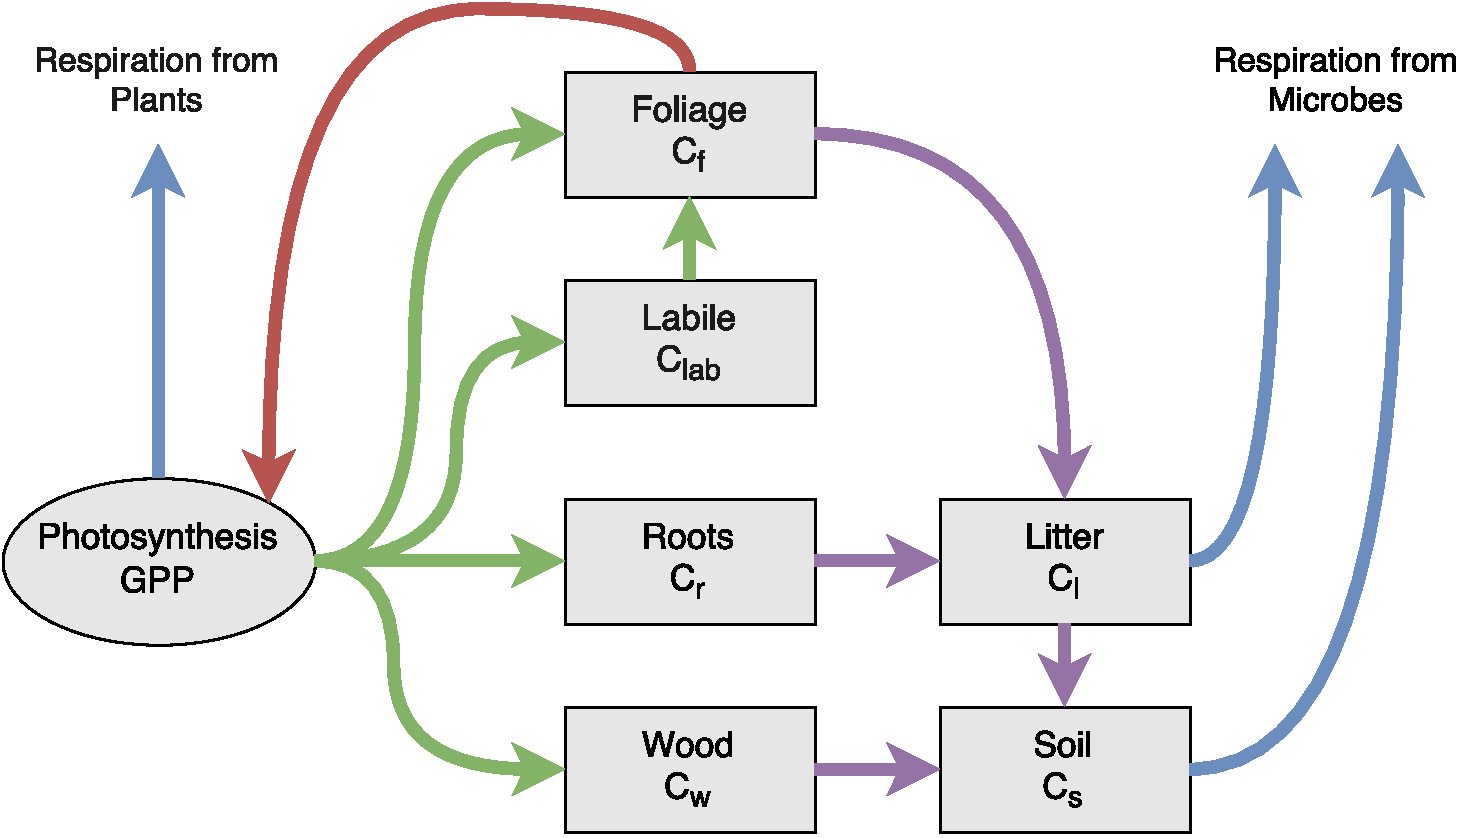
\includegraphics[width=0.5\textwidth]{DALECdiagram.pdf}
    \caption{Representation of the fluxes in the DALEC2 carbon balance model. Green arrows represent C allocation, purple arrows represent litter fall and decomposition fluxes, blue arrows represent respiration fluxes and the red arrow represents the influence of leaf area index in the $GPP$ function.}
    \label{fig:DALEC_mod}
\end{figure}

The model equations for the carbon pools at day $t+1$ are as follows:

\begin{align}
GPP^{t} &= ACM(C_f^{t}, c_{lma}, c_{eff}, \Psi) \label{GPP}
\\C_{lab}^{t+1}&=(1-\Phi _{on})C_{lab}^{t}+(1-f_{auto})(1-f_{fol})f_{lab}GPP^{t}, \label{daleclab}
\\C_f^{t+1}&=(1-\Phi_{off})C_f^{t}+\Phi_{on}C_{lab}^{t}+(1-f_{auto})f_{fol}GPP^{t}, \label{dalec1}
\\C_r^{t+1}&=(1-\theta_{roo})C_r^{t}+(1-f_{auto})(1-f_{fol})(1-f_{lab})f_{roo}GPP^{t}, 
\\C_w^{t+1}&=(1-\theta_{woo})C_w^{t}+(1-f_{auto})(1-f_{fol})(1-f_{lab})(1-f_{roo})GPP^{t}, 
\\C_l^{t+1}&=(1-(\theta_{lit}+\theta_{min})e^{\Theta T^{t}})C_l^{t}+\theta_{roo}C_r^{t}+\Phi_{off}C_f^{t}, 
\\C_s^{t+1}&=(1-\theta_{som}e^{\Theta T^{t}})C_s^{t}+\theta_{woo}C_w^{t}+\theta_{min}e^{\Theta T^{t}}C_l^{t}, \label{dalec5}
\end{align}
where $T^{t}$ is the daily mean temperature, $\Psi$ represents the meteorological driving data used in the $GPP$ function and $\Phi_{on} / \Phi_{off}$ are functions controlling leaf-on and leaf-off. The model parameters used in equations \ref{GPP} to \ref{dalec5} are included in the appendix in table~\ref{table:xbvars}. DALEC2 differs from the original DALEC in that it can be parameterised for both deciduous and evergreen sites with $\Phi_{on}$ and $\Phi_{off}$ being able to reproduce the phenology of either type of site. The full details of this version of DALEC can be found in \cite{Bloom2015}. 

\subsection{4D-Var} \label{4dvar}

In 4D-Var we aim to maximise the probability of $P(\textbf{x}_0|\textbf{y})$, the initial state $\textbf{x}_0$ given a set of observations $\textbf{y}$ over some time window, $0, \dots, N$. The probability $P(\textbf{x}_0|\textbf{y})$ is maximised by minimising a cost function $J(\textbf{x}_0)$ derived from Bayes Theorem \citep{lawless2013}. The cost function is given as,

\begin{equation}
J(\textbf{x}_0) = \frac{1}{2}(\textbf{x}_0-\textbf{x}_b)^{T}\textbf{B}^{-1}(\textbf{x}_0-\textbf{x}_b)+\frac{1}{2}\sum_{i=0}^{N}(\textbf{y}_i-h_i(\textbf{x}_i))^{T}\textbf{R}_{i}^{-1}(\textbf{y}_i-h_i(\textbf{x}_i)),
\end{equation}
where $\textbf{x}_b$ is the so-called background and acts as the initial guess to the state $\textbf{x}_0$, $\textbf{B}$ is the background error covariance matrix and quantifies our knowledge of the error in the background, $h_i$ is the observation operator at time $t_i$ and maps the state vector evolved by the nonlinear model ($m_{0\rightarrow i}(\mathbf{x}_{0})=\textbf{x}_i$) to the observations at this time ($\textbf{y}_i$) and $\textbf{R}_i$ is the observation error covariance matrix at time $t_i$ and represents our knowledge of the uncertainty in the observations. The state that minimises the cost function is called the analysis and is denoted as $\textbf{x}_a$. This state is found using a minimisation routine that takes as its input arguments the cost function, the initial guess ($\textbf{x}_b$) and also the gradient of the cost function given as,

\begin{equation}
\nabla J(\textbf{x}_0) = \textbf{B}^{-1}(\textbf{x}_0-\textbf{x}_b)-\sum_{i=0}^{N}\textbf{M}_{i,0}^{T}\textbf{H}_i^{T}\textbf{R}_{i}^{-1}(\textbf{y}_i-h_i(\textbf{x}_i)),
\end{equation}

where $\textbf{H}_i = \frac{\partial h_i(\textbf{x}_i)}{\partial\textbf{x}_i}$ is our linearized observation operator and $\mathbf{M}_{i,0}=\mathbf{M}_{i-1}\mathbf{M}_{i-2}\cdots\mathbf{M}_0$ is the tangent linear model with $\mathbf{M}_i=\frac{\partial m_{i}(\textbf{x}_{i})}{\partial \textbf{x}_{i}}$. In practice $\nabla J(\textbf{x}_0)$ is calculated using the method of Lagrange multipliers as shown in \citet{lawless2013}. We can rewrite the cost function and its gradient to avoid the sum notation as,

\begin{equation}
J(\textbf{x}_0) = \frac{1}{2}(\textbf{x}_0-\textbf{x}_b)^{T}\textbf{B}^{-1}(\textbf{x}_0-\textbf{x}_b)+\frac{1}{2}(\hat{\textbf{y}}-\hat{h}(\textbf{x}_0))^{T}\hat{\textbf{R}}^{-1}(\hat{\textbf{y}}-\hat{h}(\textbf{x}_0)) \label{costfn}
\end{equation}
and
\begin{equation}
\nabla J(\textbf{x}_0) = \textbf{B}^{-1}(\textbf{x}_0-\textbf{x}_b)-\hat{\mathbf{H}}^{T}\hat{\textbf{R}}^{-1}(\hat{\textbf{y}}-\hat{h}(\textbf{x}_0)), \label{gradcostfn}
\end{equation}
where,
\begin{equation}
\hat{\textbf{y}}=
\begin{pmatrix}
\textbf{y}_0 \\
\textbf{y}_1\\
\vdots \\
\textbf{y}_N
\end{pmatrix},
\hspace{1mm}
\hat{h}(\textbf{x}_0)=
\begin{pmatrix}
h_0(\textbf{x}_0) \\
h_1(m_{0\rightarrow 1}(\mathbf{x}_{0}))\\
\vdots \\
h_N(m_{0\rightarrow N}(\mathbf{x}_{0}))
\end{pmatrix},
\hspace{1mm}
\hat{\mathbf{R}}=
\begin{pmatrix}
\mathbf{R}_{0, 0} & \mathbf{R}_{0, 1} & \dots & \mathbf{R}_{0, N} \\
\mathbf{R}_{1, 0} & \mathbf{R}_{1, 1} & \dots & \mathbf{R}_{1, N} \\
\vdots & \vdots & \ddots & \vdots \\
\mathbf{R}_{N, 0} & \mathbf{R}_{N, 1} & \dots & \mathbf{R}_{N, N}
\end{pmatrix}
\hspace{1mm} \text{and} \hspace{3mm}
\hat{\mathbf{H}}=
\begin{pmatrix}
\mathbf{H}_0 \\
\mathbf{H}_1\mathbf{M}_0\\
\vdots \\
\mathbf{H}_N\mathbf{M}_{N,0}
\end{pmatrix}.
\end{equation}

Solving the cost function in this form also allows us to build serial correlations into the observation error covariance matrix $\hat{\mathbf{R}}$. The off-diagonal blocks of $\hat{\mathbf{R}}$ represent correlations in time between assimilated observations and are usually taken to be zero.
%Forecast skill score, $SS = 1 - \frac{MSE_{forecast}}{MSE_{ref}}$, http://en.wikipedia.org/wiki/Forecast_skill

\subsection{Implementation and testing of 4D-Var system}

In our DALEC2 4D-Var scheme we are performing joint parameter and state estimation. Therefore the state vector, $\textbf{x}_0$, corresponds to the vector of the 17 model parameters and 6 initial carbon pool values, which can be found in the appendix in table~\ref{table:xbvars}. Here the nonlinear model (DALEC2) only updates the initial carbon pool values when evolving the state vector forward in time with the parameters being held constant. To find the background guess, $\textbf{x}_{b}$, to the state vector we can either use a previous DALEC2 model forecast's estimate to the state of the system for the site (when available) or use expert elicitation to define likely state and parameter values and ranges for the site. The background vector $(\textbf{x}_b)$ and its corresponding standard deviations (see table~\ref{table:xbvars}) used in this paper were provided from existing runs of the the CARbon DAta-MOdel fraMework (CARDAMOM) \citep{Exbrayat2015}. This is a worse resolution dataset which provides a reasonable first guess at DALEC2 state and parameter values for the Alice Holt research site.

In order to find the tangent linear model (TLM) for DALEC2 it is necessary to find the derivative of the model at each time step with respect to the 17 model parameters and the 6 carbon pools. We use the AlgoPy automatic differentiation package \citep{Walter2013} in Python to calculate the TLM at each time step. This package uses forward mode automatic differentiation to calculate the derivative of our model. In the following tests we use a diagonal approximation to our background and observational error covariance matrices so that, 
$\textbf{B}_{diag}=\text{diag}(\bm{\sigma}_b)^2$ and $\hat{\textbf{R}}_{diag}=\text{diag}(\bm{\sigma}_o )^2$,
where $\bm{\sigma}_b$ and $\bm{\sigma}_o$ are the vectors of the background and observational standard deviations respectively. 

In this paper we assimilate observations of daily NEE. The flux tower actually produces an estimate of NEE every half-hour. We take the sum over the 48 measurements made each day. We only select days where there is no missing data and over $90\% $ of observations have a quality control flag associated with the best observations from the EddyPro flux processing software \citep{eddypro}. We take a variance of $0.5\text{gCm}^{-2}\text{day}^{-1}$ in our assimilated observations of daily NEE \citep{williams2005improved}. The minimisation routine used in our data assimilation experiments is the truncated Newton method \citep{Nocedal1999} from the Python package Scipy.optimize. In sections \ref{sec:testtlm} to \ref{sec:testgrad} we show tests of our scheme. 


\subsubsection{Test of tangent linear model} \label{sec:testtlm}

We can have confidence that our implementation of the TLM for DALEC2 is correct as it passes the following relevant tests \citep{Li1994}. In 4D-Var we assume the tangent linear hypothesis,
\begin{equation}
m_{0\rightarrow i}(\mathbf{x}_0+\gamma \delta\mathbf{x}_0) \approx m_{0 \rightarrow i}(\mathbf{x}_0) + \mathbf{M}_{i,0}\gamma \delta\mathbf{x}_0, \label{TLH}
\end{equation}
where $\delta\mathbf{x}_0$ is a perturbation of the initial state and $\gamma$ is a parameter controlling the size of this perturbation. The validity of this assumption depends on how nonlinear the model is, the length of the assimilation window and the size of the perturbation $\delta\mathbf{x}_0$. We can test this by rearranging equation~\ref{TLH} to find the relative error,
\begin{equation}
E_R=\frac{||m_{0\rightarrow i}(\mathbf{x}_0+\gamma \delta\mathbf{x}_0) - m_{0 \rightarrow i}(\mathbf{x}_0)||}{||\mathbf{M}_{i,0}\gamma\delta\mathbf{x}_0||}, \label{tlmtest}
\end{equation}
where we expect $E_R \rightarrow 0$ as $\gamma \rightarrow 0$ (here we are using the Euclidean norm). Figure~\ref{fig:tlm} shows equation~\ref{tlmtest} plotted for DALEC2 with a TLM evolving our state 731 days forward in time for different values $\gamma$, with a $5\%$ perturbation $\delta\mathbf{x}_0$. Figure~\ref{fig:tlm} shows that the TLM behaves as expected for values of $\gamma$ approaching $0$.


\begin{figure}[ht]
    \centering
    \includegraphics[width=0.5\textwidth]{linmoderr.eps}
    \caption{Plot of the tangent linear model test function (equation \ref{tlmtest}) for DALEC2, for a TLM evolving our state 731 days forward in time and a $5\%$ perturbation, $\delta \textbf{x}_0$.}
    \label{fig:tlm}
\end{figure}

It is also useful to show how our TLM behaves over a time window to see how the error in the TLM grows as we evolve our state further forward in time. We again rearrange equation \ref{TLH} with an additional error term to find, 
\begin{equation}
\text{percentage error in TLM} = \begin{vmatrix} \frac{||m_{0\rightarrow i}(\mathbf{x}_0+\delta\mathbf{x}_0) - m_{0 \rightarrow i}(\mathbf{x}_0)||}{|| \mathbf{M}_{i,0}\delta\mathbf{x}_0||} - 1 \end{vmatrix} \times 100. \label{pertlmtest}
\end{equation}

\begin{figure}[ht]
    \centering
    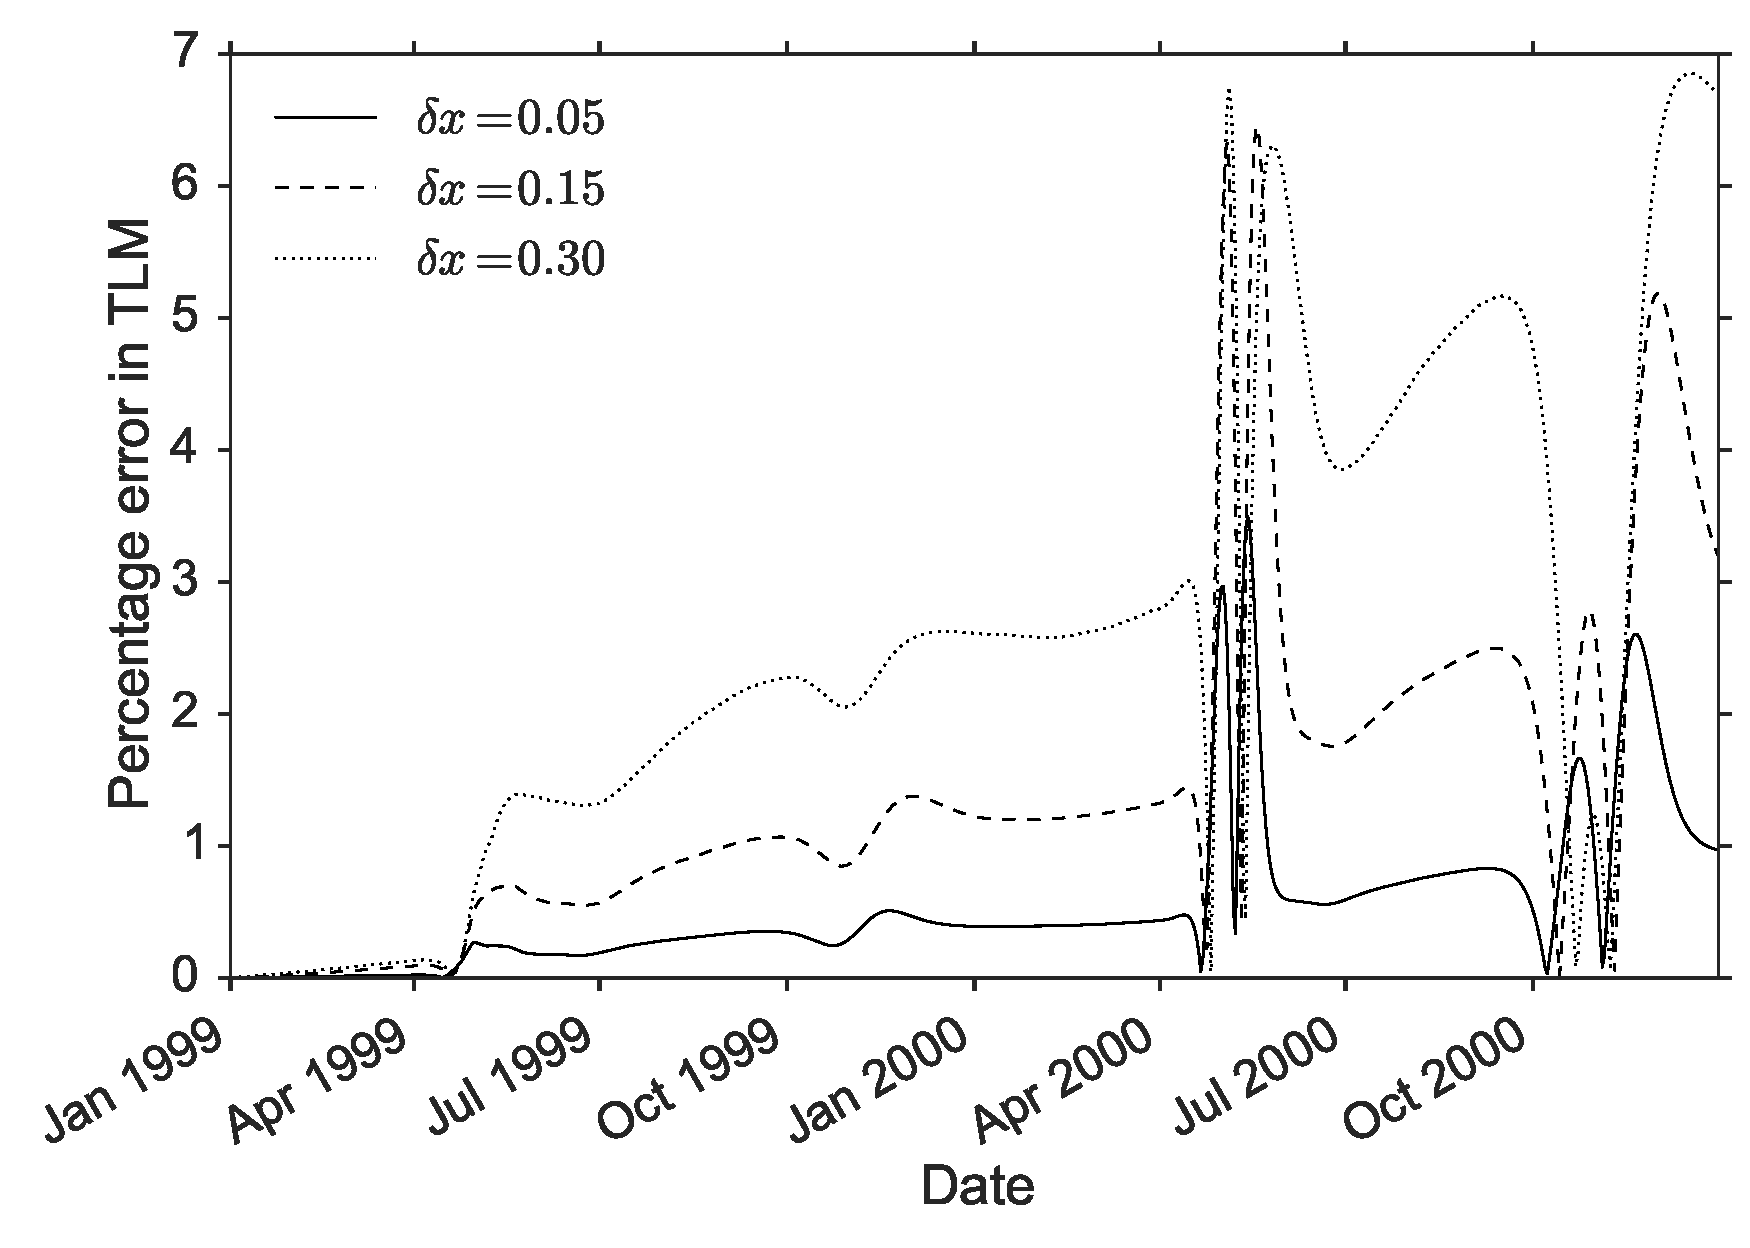
\includegraphics[width=0.5\textwidth]{percenterrlinmod.eps}
    \caption{Plot of the percentage error in the tangent linear model (equation \ref{pertlmtest}) for DALEC2 when evolving the model state forward over a period of two years with three differing values of perturbation, $\delta \textbf{x}_0$.}
    \label{fig:tlm_error}
\end{figure}

In figure \ref{fig:tlm_error} we can see that our TLM for DALEC2 performs well after being run forward a year with less than a $3\%$ error for all values of $\delta \textbf{x}_0$. By the second year we see some peaks in our error in spring and autumn. This is due to leaf on and leaf off functions in the TLM going out of phase with the nonlinear DALEC2. Even at these peaks our error is still reasonable reaching a maximum at $7\%$ and then coming back to around $1\%$. For this reason we present results using a one year assimilation window in this paper. 

\subsubsection{Test of adjoint model} 

The adjoint model we have implemented for DALEC2 passes correctness tests. For our TLM $\mathbf{M}_{i,0}$ and its adjoint $\mathbf{M}_{i,0}^{T}$ we have the identity
\begin{equation}
<\mathbf{M}_{i,0}\delta\textbf{x}_0, \mathbf{M}_{i,0}\delta\textbf{x}_0> = <\delta\textbf{x}_0, \mathbf{M}_{i,0}^{T}\mathbf{M}_{i,0}\delta\textbf{x}_0> \label{eqn:adjoint_test}
\end{equation}
for any inner product $<, >$ and perturbation $\delta \textbf{x}_0$, this is derived from the adjoint identity \citep{lawless2013}. Using the Euclidean inner product equation~\ref{eqn:adjoint_test} is equivalent to
\begin{equation}
(\mathbf{M}_{i,0}\delta\textbf{x}_0)^{T} (\mathbf{M}_{i,0}\delta\textbf{x}_0) = \delta\textbf{x}_0^{T} (\mathbf{M}_{i,0}^{T}(\mathbf{M}_{i,0}\delta\textbf{x}_0)).
\end{equation}
We evaluated the left hand side and right hand side of this identity for differing values of $\delta \textbf{x}_0$ and showed that they were equal to machine precision.

\subsubsection{Gradient test} \label{sec:testgrad}

The 4D-Var system we have developed passes tests for the gradient of the cost function \citep{Navon1992}. In the implementation of the cost function and its gradient we regularise the problem using a variable transform \citep{Freitag2010}. For our cost function $J$ and its gradient $\nabla J$ we can show that we have implemented $\nabla J$ correctly using the identity,
\begin{equation}
f(\alpha)=\frac{| J( \textbf{x}_0 + \alpha \textbf{b}) - J(\textbf{x}_0) |}{\alpha \textbf{b}^{T} \nabla J(\textbf{x}_0)} = 1 + O(\alpha),
\end{equation}
where $\textbf{b}$ is a vector of unit length and $\alpha$ is a parameter controlling the size of $\textbf{b}$. For small values of $\alpha$ not too close to machine precision we should have $f(\alpha)$ close to 1. Figure~\ref{fig:costone} shows $f(\alpha)$ for a 365 day assimilation window with $\textbf{b}=\textbf{x}_0||\textbf{x}_0||^{-1}$, we can see that $f(\alpha) \rightarrow 1$ as $\alpha \rightarrow 0$, as expected until $f(\alpha)$ gets too close to machine zero at $O(\alpha) = 10^{-11}$.

We can also plot $|f(\alpha)-1|$, where we expect $|f(\alpha)-1| \rightarrow 0$ as $\alpha \rightarrow 0$.  In figure~\ref{fig:cost} we have plotted $|f(\alpha)-1|$ for the same conditions as in figure~\ref{fig:costone}, we can see that $|f(\alpha) - 1| \rightarrow 0$ as $\alpha \rightarrow 0$, as expected (before $|f(\alpha)-1|$ gets too close to machine precision at $O(\alpha) = 10^{-8}$). This gives us confidence that the gradient of our cost function is implemented correctly.
%$\nabla J(\textbf{x}_0)||\nabla J(\textbf{x}_0)||^{-1}$. 

\begin{figure}[ht]
    \centering
    \begin{subfigure}[b]{0.49\textwidth}
        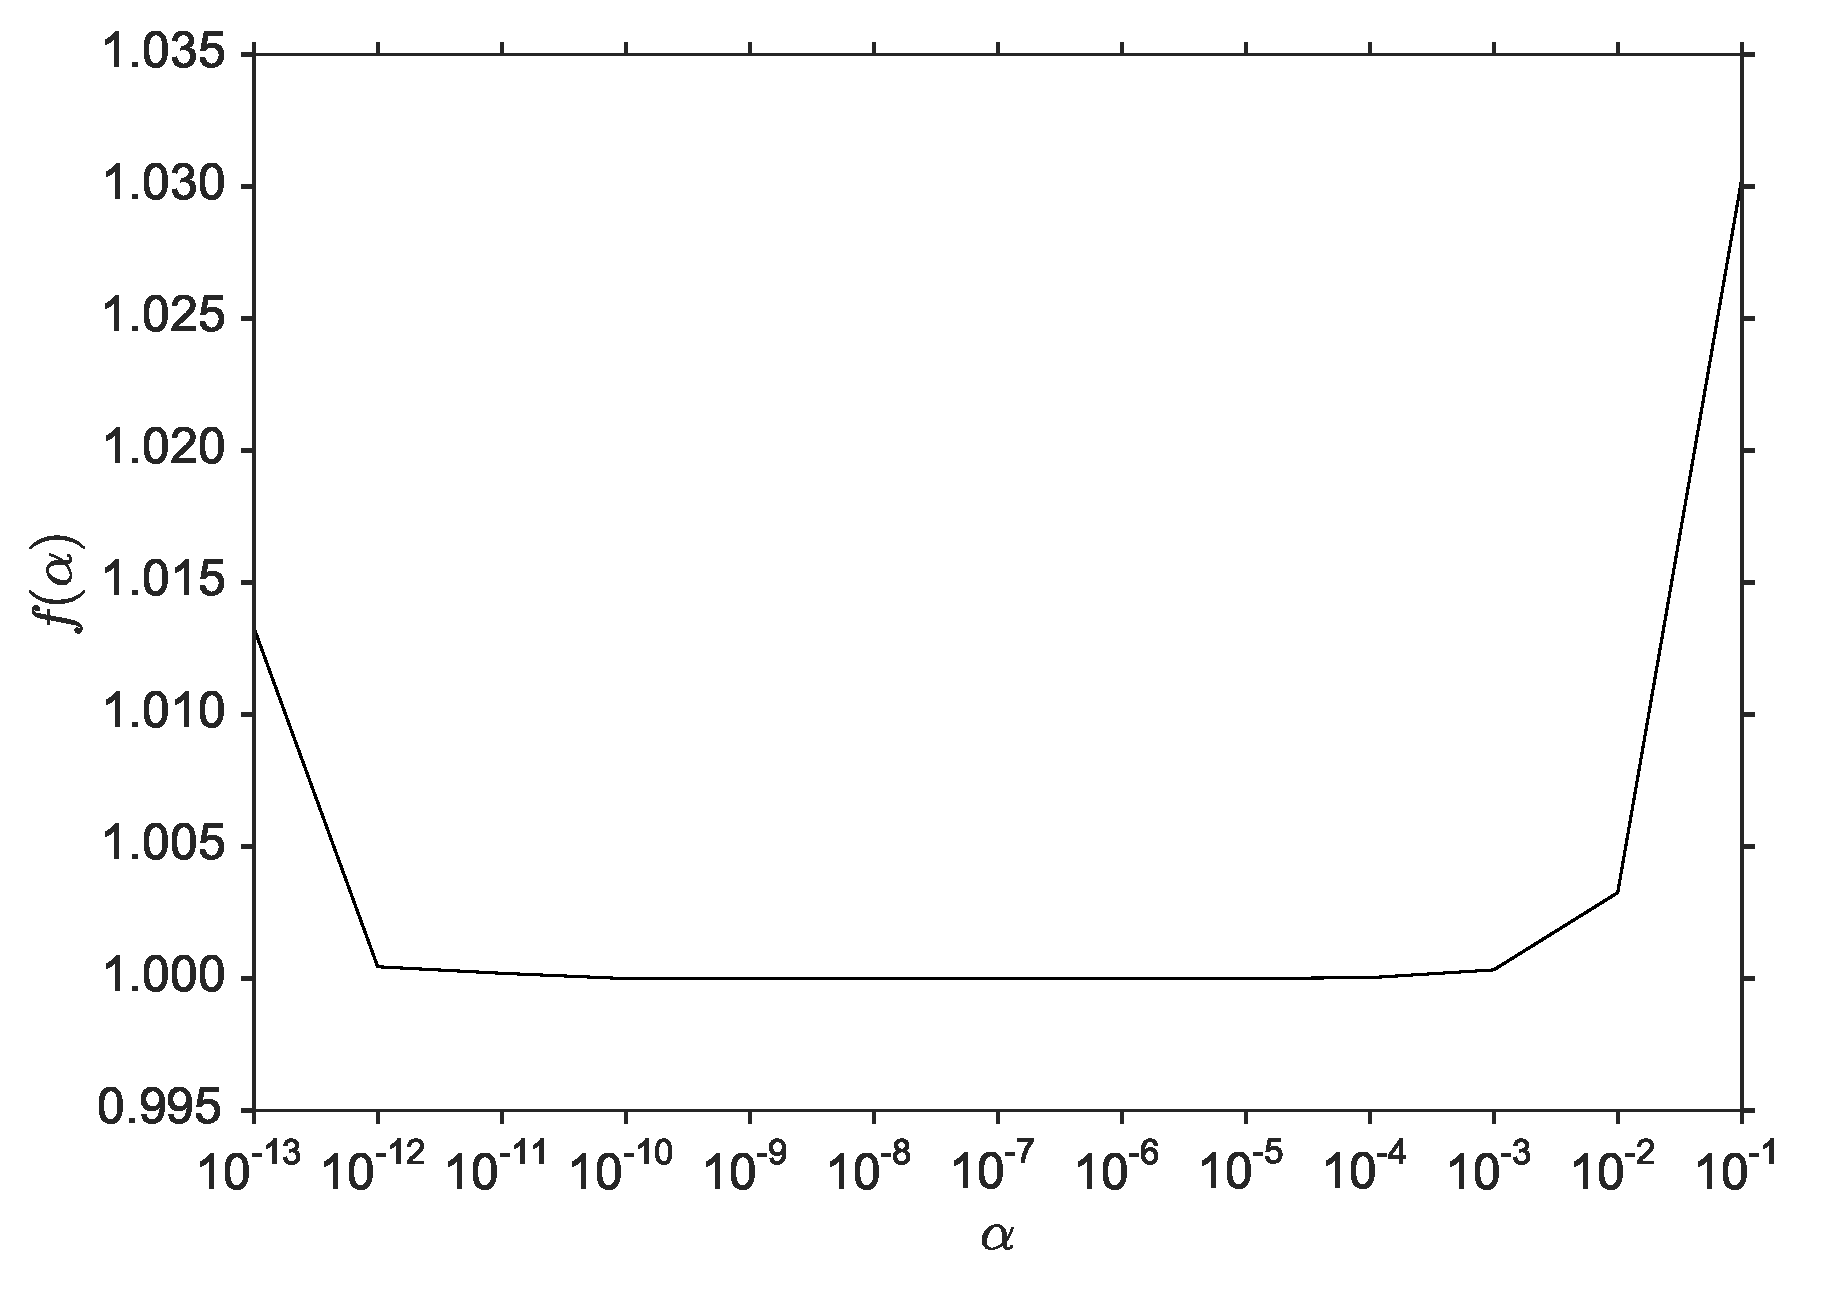
\includegraphics[width=\textwidth]{costone_cvt.eps}
        \caption{$f(\alpha)$ test}
        \label{fig:costone}
    \end{subfigure}
    \begin{subfigure}[b]{0.49\textwidth}
        \includegraphics[width=\textwidth]{cost_cvt.eps}
        \caption{$|f(\alpha) - 1|$ test}
        \label{fig:cost}
    \end{subfigure}
    \caption{Tests of the gradient of the cost function for a 365 day assimilation window with $\textbf{h}=\textbf{x}_0||\textbf{x}_0||^{-1}$.}
    \label{fig:testgradcostone}
\end{figure}

\subsection{Including correlations in the background error covariance matrix} \label{sec:corB}

As discussed in section~\ref{sec:intro}, including correlations in \textbf{B} impacts how information from assimilated observations is spread between different types of analysis variables \citep{bannister2008review}. We explored a number of different methods in order to include parameter-state correlations in \textbf{B}. In this paper we present a method using a set of ecological dynamical constraints on model parameters and state variables from \citet{Bloom2015}. In \citet{Bloom2015} implementing these constraints in a Metropolis Hastings MCMC data assimilation routine is shown to improve results significantly. The constraints impose conditions on carbon pool turnover and allocation ratios, steady state proximity and growth and decay of model carbon pools.

In order to create a correlated background error covariance matrix, $\textbf{B}_{corr}$, using these constraints we create an ensemble of state vectors which we then take the covariance of to give us $\textbf{B}_{corr}$. To create this ensemble we use the following procedure:
\begin{enumerate}
\item Draw a random state vector, $\textbf{x}_i$, from the multivariate truncated normal distribution described by our $\textbf{x}_b$, associated variances and parameter-state ranges given in table~\ref{table:xbvars}.
\item Test this $\textbf{x}_i$ with the ecological dynamical constraints (requiring us to run the DALEC2 model using this state).
\item If $\textbf{x}_i$ passes it is added to to our ensemble, else it is discarded.
\end{enumerate}
Once we have a full ensemble (we chose an ensemble size of 1500 as past this point values of correlations did not appear to change significantly) we then take the covariance of the ensemble to find $\textbf{B}_{corr}$. In figure \ref{fig:Bcorr} we have plotted the correlation matrix or normalised error covariance matrix of $\textbf{B}_{corr}$. This matrix includes both positive and negative correlations between parameter and state variables, with correlations of 1 down the diagonal between variables of the same quantity as expected. The largest positive off-diagonal correlation being $0.42$ between $f_{lab}$ and $C_{lab}$. This makes physical sense as $f_{lab}$ is the parameter controlling the amount of GPP allocated to the labile carbon pool, $C_{lab}$.

\begin{figure}[ht]
    \centering
    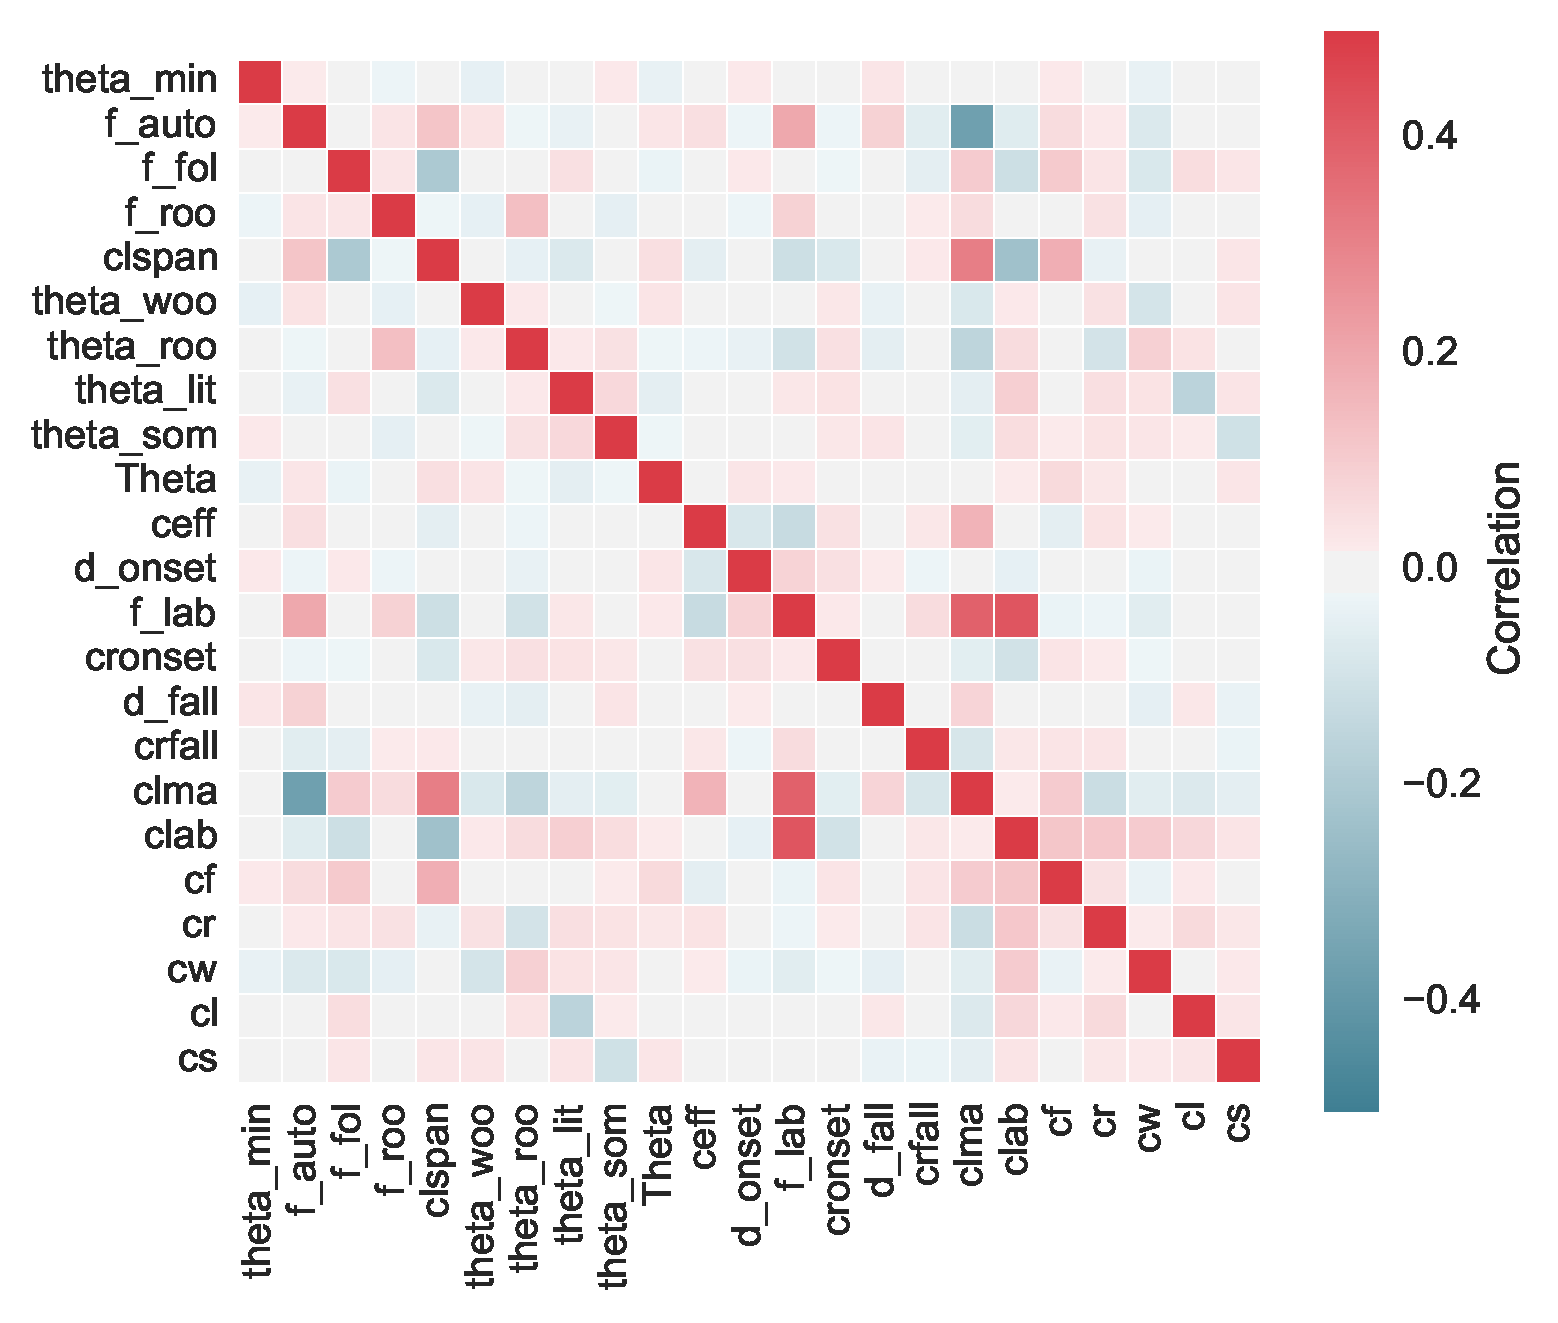
\includegraphics[width=0.55\textwidth]{bedccor.eps}
    \caption{Background error correlation matrix created using method in section \ref{sec:corB}}
    \label{fig:Bcorr}
\end{figure}

\subsection{Specifying serial correlations in the observational error covariance matrix} \label{sec:corR}

Errors in NEE observations come from different sources such as instrument errors, sampled ecosystem structure and turbulent conditions (when we have low turbulence and limited air mixing NEE is underestimated) \citep{Papale2006}. Due to this dependance on atmospheric conditions we expect the errors in observations of NEE to be serially correlated, as the atmospheric signal itself is serially correlated \citep{Daley1992}. If we were assimilating half hourly observations of NEE we would expect stronger correlations between observation errors, as atmospheric conditions are more constant at this time scale, with correlations between observation errors getting weaker with lower frequency observations. The observation error covariance matrix does not only represent the instrumentation error for an observation but also the error in the observation operator (mapping the model state to the observation) and representativity error (error arising from the model being unable resolve the spatial and temporal scales of the observations). These other sources of error represented in $\hat{\textbf{R}}$ can also lead to correlations between observation errors \citep{Waller2014}.   

In section~\ref{4dvar} we have re-written the 4D-Var cost function in equation~\ref{costfn} in order to allow the specification of serial observation error correlations in our assimilation scheme. These serial correlations are represented by the off-diagonal blocks of $\hat{\mathbf{R}}$. In work carried out with spatial correlations it has been shown that the structure of the correlation is not critical \citep{Healy2005} and that it is better to include some estimate of error correlation structure in the observation error covariance matrix than wrongly assume that errors are independent \citep{Stewart2013}. As a first attempt we try including correlations on the scale of the observation frequency. We adapt the simple Gaussian model found in \citet{jarvinen1999variational} (a second order autoregressive correlation function was also tested but not presented here). The correlation $r$ between 2 observations at times $t_1$ and $t_2$ is given as,
\begin{equation}
r =
\begin{cases} 
      a \text{exp} \bigg[ \frac{-(t_1 - t_2)^2}{\tau^2} \bigg] + (1- a)\delta_{t_1 - t_2} & |t_1 - t_2| \leq \eta \\
      0 & \eta < |t_1 - t_2| 
   \end{cases}
   , \label{eqn:corr_fn}
\end{equation}
where $\tau$ is the e-folding time, $a$ controls the strength of correlation, $\delta$ is the Kronecker delta and $\eta$ is the cut off time after which the correlation between two observation errors is zero. We have incorporated a cut off for correlations between observation errors as the assumed correlation length scale for our assimilated observations is short. This cut off along with the form of correlation function using the Kronecker delta helps ensure $\hat{\mathbf{R}}$ is positive definite and therefore invertible, as required in the assimilation process. 

\begin{figure}[ht]
    \centering
    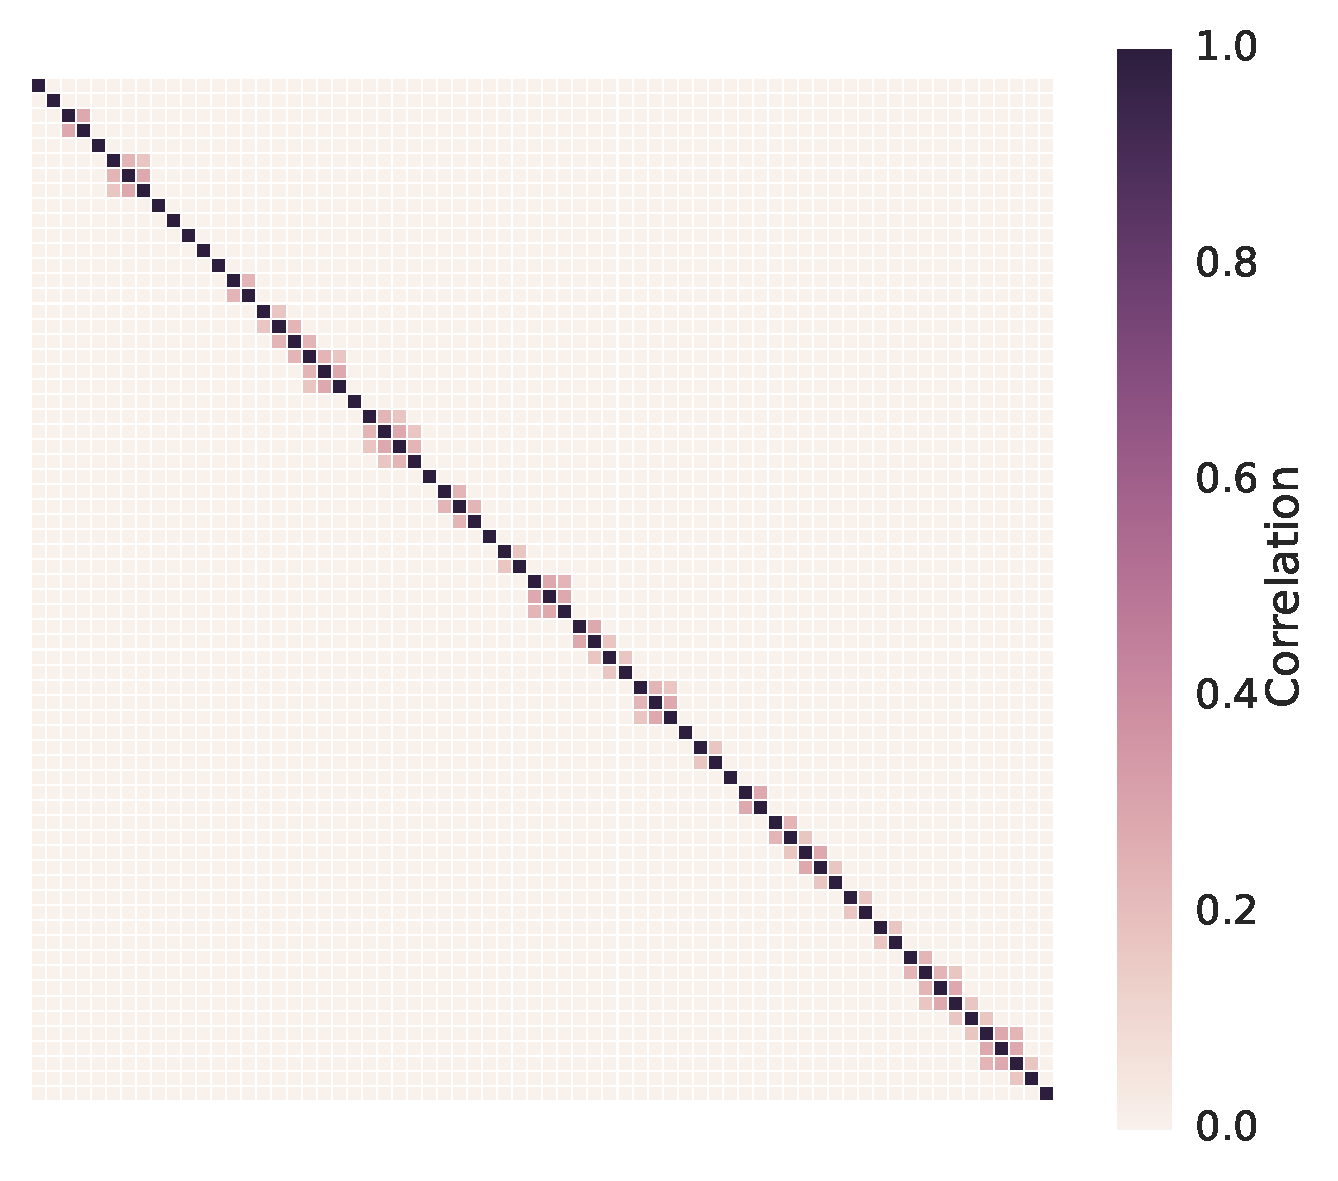
\includegraphics[width=0.5\textwidth]{rcorcor.eps}
    \caption{Observation error correlation matrix for the 67 observations used in assimilation created using method in section \ref{sec:corR} with $\tau = 4$, $a=0.3$ and $\eta=4$.}
    \label{fig:Rcorr}
\end{figure}

Figure~\ref{fig:Rcorr} shows the correlation matrix for $\hat{\mathbf{R}}$ created using equation~\ref{eqn:corr_fn}, there are 67 NEE observations in this one year assimilation window, these observations are not all on adjacent days and this is evident in the structure of $\hat{\mathbf{R}}$. The effect of the short e-folding time chosen here ($\tau=4$) provides the desired structure. 

\section{Results} \label{sec:results}

\subsection{Experiments} \label{sec:exps}

In the following sections we present the results of 4 experiments where we vary the representations of $\textbf{B}$ and $\hat{\mathbf{R}}$ while assimilating the same NEE observations in the window from 1999-2000. As shown in figure~\ref{fig:tlm_error} the performance of the tangent linear model deteriorates after the first year. We then forecast the NEE over the next 14 years and compare with the observed data. These experiments are outlined in table~\ref{table:exps_tab} where $\textbf{B}_{diag}$ and $\hat{\mathbf{R}}_{diag}$ are the diagonal matrices of the parameter-state variances and the observations variances respectively and $\textbf{B}_{corr}$ and $\hat{\mathbf{R}}_{corr}$ are the matrices as specified in section~\ref{sec:corB} and section~\ref{sec:corR} respectively.

\begin{table}[ht] 
\begin{center}
	\begin{tabular}{| l | l | l | l | l |}
	\hline
	Experiment & $\textbf{B}_{diag}$ & $\hat{\mathbf{R}}_{diag}$ & $\textbf{B}_{corr}$ &
	$\hat{\mathbf{R}}_{corr}$ \\ \hline
	A & $\times$ & $\times$ & & \\ \hline
	B & & $\times$ & $\times$ & \\ \hline
	C & $\times$ & & & $\times$ \\ \hline
	D & & & $\times$ & $\times$ \\ 
	\hline
	\end{tabular}
	\caption{The combination of error covariance matrices used in each data assimilation experiment.}
	\label{table:exps_tab}
\end{center} 
\end{table}

\subsection{Experiment A} \label{sec:expa}
In this experiment $\textbf{B}_{diag}$ and $\hat{\textbf{R}}_{diag}$ were used in our assimilation as described in section~\ref{sec:exps}. Because these contain no correlations this experiment forms the baseline by which the subsequent results from assimilation experiments are judged.  

Figure~\ref{fig:4dvardiagBR} shows assimilation and forecast results for NEE. We can see that assimilating the observations of NEE has improved the background with our analysis trajectory (green line) fitting well with the observations during the assimilation window (1999-2000). The analysis trajectory then diverges in the forecast (2000-2014). This can be seen more clearly in figue~\ref{fig:broke4dvardiagBR}, where we have an over prediction of respiration in the winter and the seasonal cycle does not match that of the observations. As discussed in section~\ref{sec:intro} previous work has shown the importance of specifying parameter-state correlations when using variational data assimilation for joint parameter-state estimation \citep{smith2009variational}. Although in 4D-Var some correlation structure is added implicitly as $\textbf{B}_{diag}$ is evolved through time, observations near the beginning of the window (before significant correlations develop in $\textbf{B}_{diag}$) will not be spread in a multivariate way. The correlations developed by the implicit evolution of $\textbf{B}_{diag}$ may also not include important physical relationships between variables. Therefore by not specifying these correlations in this experiment we allow our parameter and state variables to attain unrealistic values in order to find the best fit to the observations in the analysis window (1999-2000), leading to the divergence seen in the forecast (1999-2014). 

To see how well our forecast performs after assimilation we show a scatter plot of modelled NEE against observed NEE in figure~\ref{fig:forecastscatBR}. Here we have a Root-Mean-Square Error (RMSE) of $4.22 \text{gCm}^{-2}$ and a bias of $-0.3 \text{gCm}^{-2}$ for our forecast of NEE, whereas our analysis (1999-2000) has a RMSE of $1.36 \text{gCm}^{-2}$ and a bias of $-0.03 \text{gCm}^{-2}$. The background trajectory meanwhile has a RMSE of $3.86 \text{gCm}^{-2}$ and a bias of $-1.60 \text{gCm}^{-2}$ in the analysis window (1999-2000) and the same RMSE of $3.86 \text{gCm}^{-2}$ but a bias of $-1.36 \text{gCm}^{-2}$ during the forecast period (2000-2014). Although using $\textbf{B}_{diag}$ and $\hat{\textbf{R}}_{diag}$ in our assimilation has considerably reduced the RMSE in our analysis period, it has also increased the RMSE in our forecast of NEE. However it has reduced the bias in the model forecast considerably from $-1.36 \text{gCm}^{-2}$ to $-0.3 \text{gCm}^{-2}$. The bias in the background comes from a constant under prediction of the more extreme negative values of NEE and this leads to considerably worse results than our analysis and its forecast for total forest carbon uptake. 

%{\color{red} **Maybe include something about the estimated reduction in error for parameter and state variables using the diagonal terms of \textbf{B} and \textbf{A} (analysis error covariance matrix). How best to compare and present these?}

\subsection{Experiment B} \label{sec:expb}

Here $\textbf{B}_{corr}$ (as defined in section~\ref{sec:corB}) and $\hat{\textbf{R}}_{diag}$ are used in our assimilation. Figure~\ref{fig:4dvaredcBR} shows assimilation and forecast results for NEE. In figure~\ref{fig:broke4dvaredcBR} we can see that the forecast performs considerably better than in experiment A, with the analysis trajectory no longer over predicting winter respiration and matching the observed seasonal cycle of NEE more closely in the forecast period (2000-2014). From figure~\ref{fig:forecastscatedcBR} and table~\ref{table:forecast_res} we see that our forecasts RMSE has almost halved (now $2.56 \text{gCm}^{-2}$) with a reduction in bias also, now $-0.2 \text{gCm}^{-2}$. In comparison using $\textbf{B}_{corr}$ in our assimilation very slightly degrades the fit for our analysis (1999-2000), with a RMSE of $1.42 \text{gCm}^{-2}$ and a bias of $-0.04 \text{gCm}^{-2}$, as shown in table~\ref{table:analysis_res}. 

We can see the effect that including correlations in $\textbf{B}$ has on the analysis update in figure~\ref{fig:xa_inc}. For some variables including correlations in $\textbf{B}$ has had a large impact on the analysis update after assimilation. This is particularly clear for the $f_{lab}$ parameter. The largest positive off-diagonal correlation in $\textbf{B}_{corr}$ is between $C_{lab}$ and $f_{lab}$, with $f_{lab}$ also having a large positive correlation with $c_{lma}$ as shown in section~\ref{sec:corB}. The effect of these correlations has been to change the analysis increment for $f_{lab}$ from being slightly positive in experiment A to being strongly negative by following the analysis update of its correlated variables $C_{lab}$ and $c_{lma}$. The added constraint provided by the correlations in $\textbf{B}_{corr}$ reduces the likelihood that parameter and state variables will attain unrealistic values in order to fit the assimilated observations. Although this has led to a slightly degraded fit to the observations in the analysis window (1999-2000) it has also significantly improved the fit to observations for the forecast (1999-2014).

%This is because our assimilation scheme is now more constrained by the background than in experiment A. Therefore using $\textbf{B}_{corr}$ in our assimilation reduces the problem of overfitting to our assimilated observations of NEE as seen in experiment A. Another improvement made by using $\textbf{B}_{corr}$ in our assimilation is that our minimisation routine converges to a solution more quickly, taking 218 fewer function iterations than experiment A to converge. 

\subsection{Experiment C} \label{sec:expc}

Here we use $\textbf{B}_{diag}$ and $\hat{\textbf{R}}_{corr}$ (as defined in section~\ref{sec:corR}) in the assimilation. Results shown in figure~\ref{fig:4dvarBcorR} and \ref{fig:broke4dvarBcorR} appear similar to those in section~\ref{sec:expa} however there are some differences. From table~\ref{table:forecast_res} and figure~\ref{fig:forecastscatBcorR} we see a slight reduction in RMSE for our forecast (now $4.09 \text{gCm}^{-2}$) in comparison with experiment A. As in experiment B the fit to the observations in the analysis window (1999-2000) is very slightly degraded as the added correlations in $\hat{\textbf{R}}_{corr}$ act to reduce the weight of the observations in the assimilation \citep{jarvinen1999variational}. The changes seen when using $\hat{\textbf{R}}_{corr}$ in the assimilation are less than when using $\textbf{B}_{corr}$ as the correlations specified in $\hat{\textbf{R}}_{corr}$ are on a short timescale and smaller than those in $\textbf{B}_{corr}$, the background error covariance matrix also plays a larger role in the assimilation spreading information between parameter and state variables \citep{bannister2008review}. In figure~\ref{fig:xa_inc} we can see that the changes between experiment A and C in the analysis increment are much less than when using $\textbf{B}_{corr}$.  

We also expect that specifying correlations in $\hat{\textbf{R}}$ will help when assimilating other less frequently sampled data streams along with NEE as the serial correlations reduce the weight given to the mean of the observations and also reduce the information content of the data streams with more observations \citep{jarvinen1999variational, Daley1992}.

\subsection{Experiment D}

In the final experiment we use $\textbf{B}_{corr}$ and $\hat{\textbf{R}}_{corr}$ in the assimilation. Figure~\ref{fig:4dvaredcBcorR} and figure~\ref{fig:4dvaredcBcorR} shows that using both correlated matrices gives similar results as experiment B when $\textbf{B}_{corr}$ is used with $\hat{\textbf{R}}_{diag}$. However using $\hat{\textbf{R}}_{corr}$ in addition to $\textbf{B}_{corr}$ provides similar improvements as in experiment C. From table~\ref{table:forecast_res} and figure~\ref{fig:forecastscatedcBcorR} we see the forecast RMSE is reduced again still from results in experiment B to $2.38 \text{gCm}^{-2}$. Using both matrices appears to combine the beneficial effects described in both section~\ref{sec:expb} and section~\ref{sec:expc}. In figure~\ref{fig:xa_inc} we can see that the analysis increment is very similar to experiment B.

\begin{figure}
    \centering
    \begin{subfigure}[b]{0.49\textwidth}
        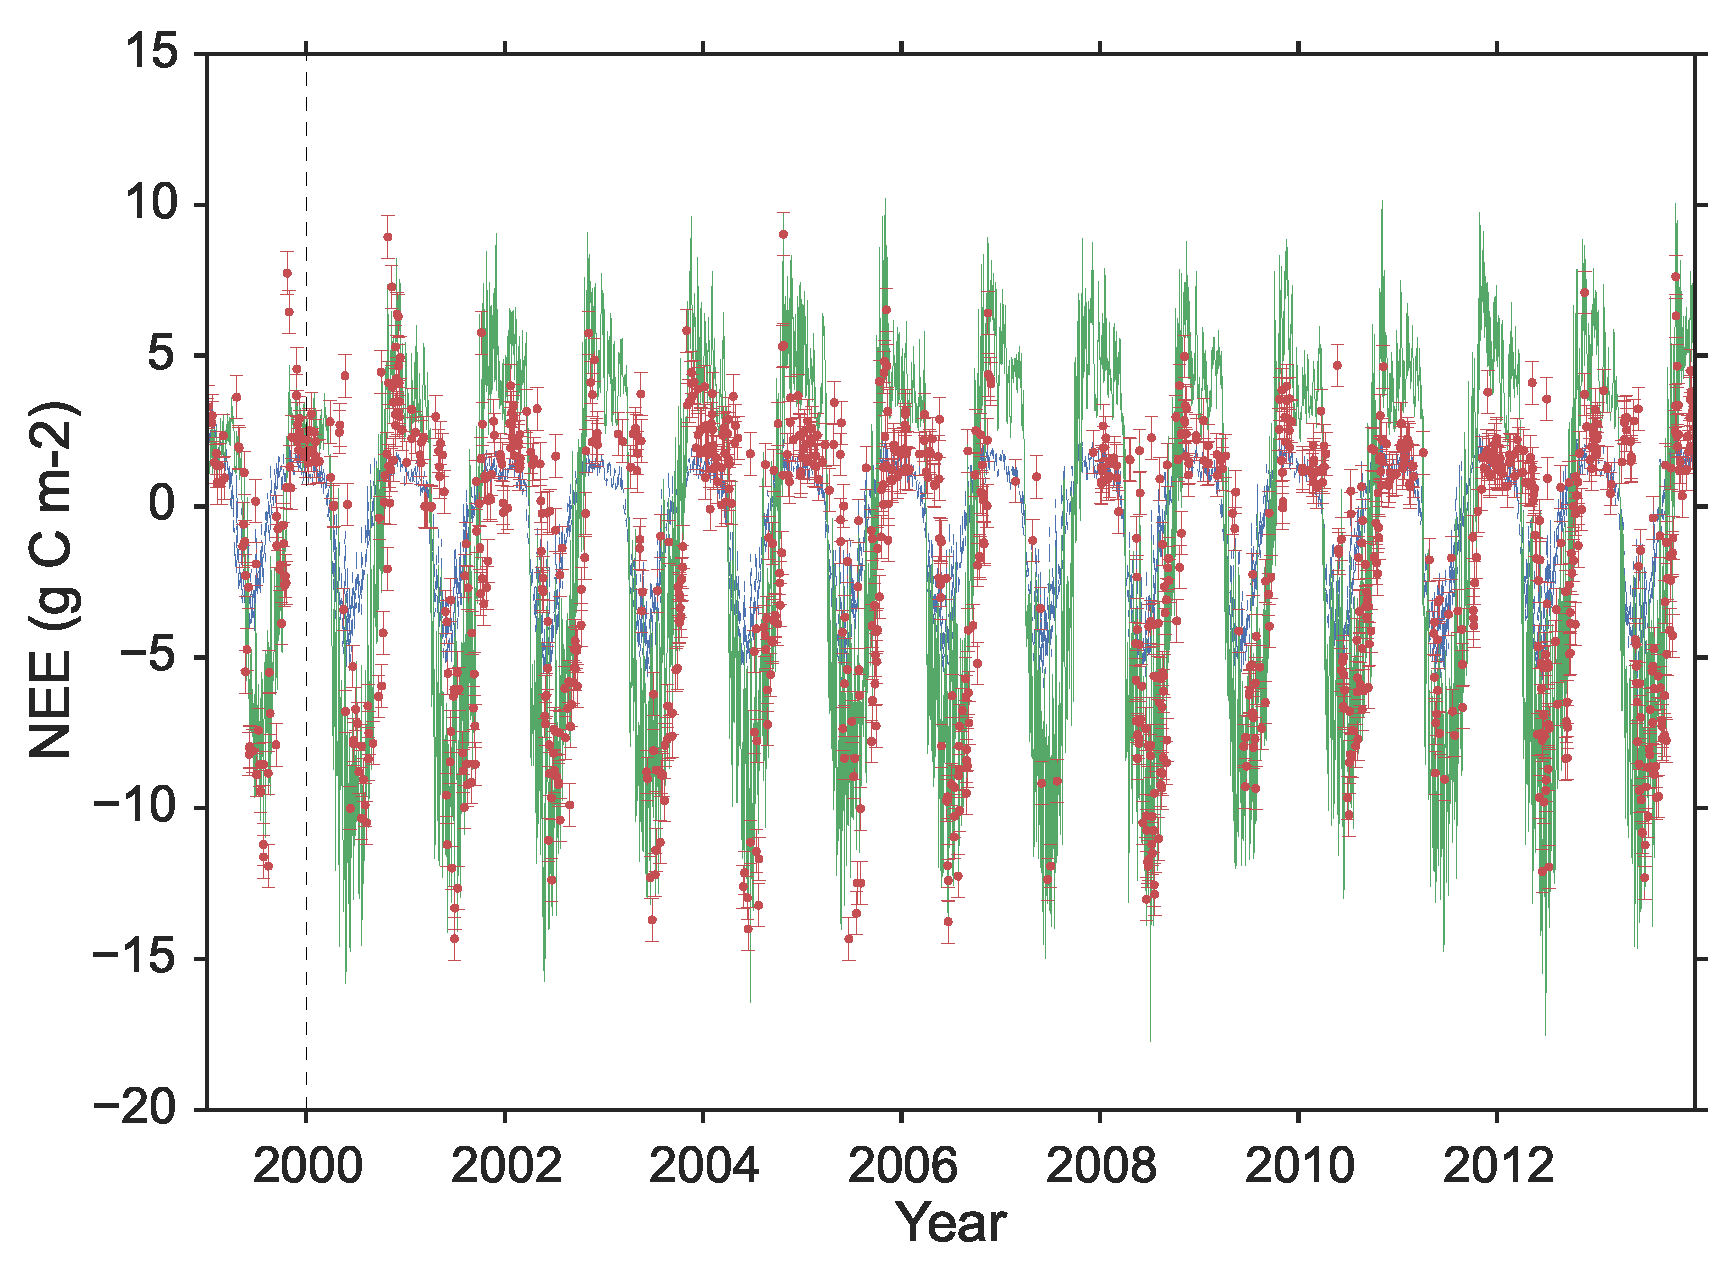
\includegraphics[width=\textwidth]{A4dvar.eps}
        \caption{Experiment A}
        \label{fig:4dvardiagBR}
    \end{subfigure}
    \begin{subfigure}[b]{0.49\textwidth}
        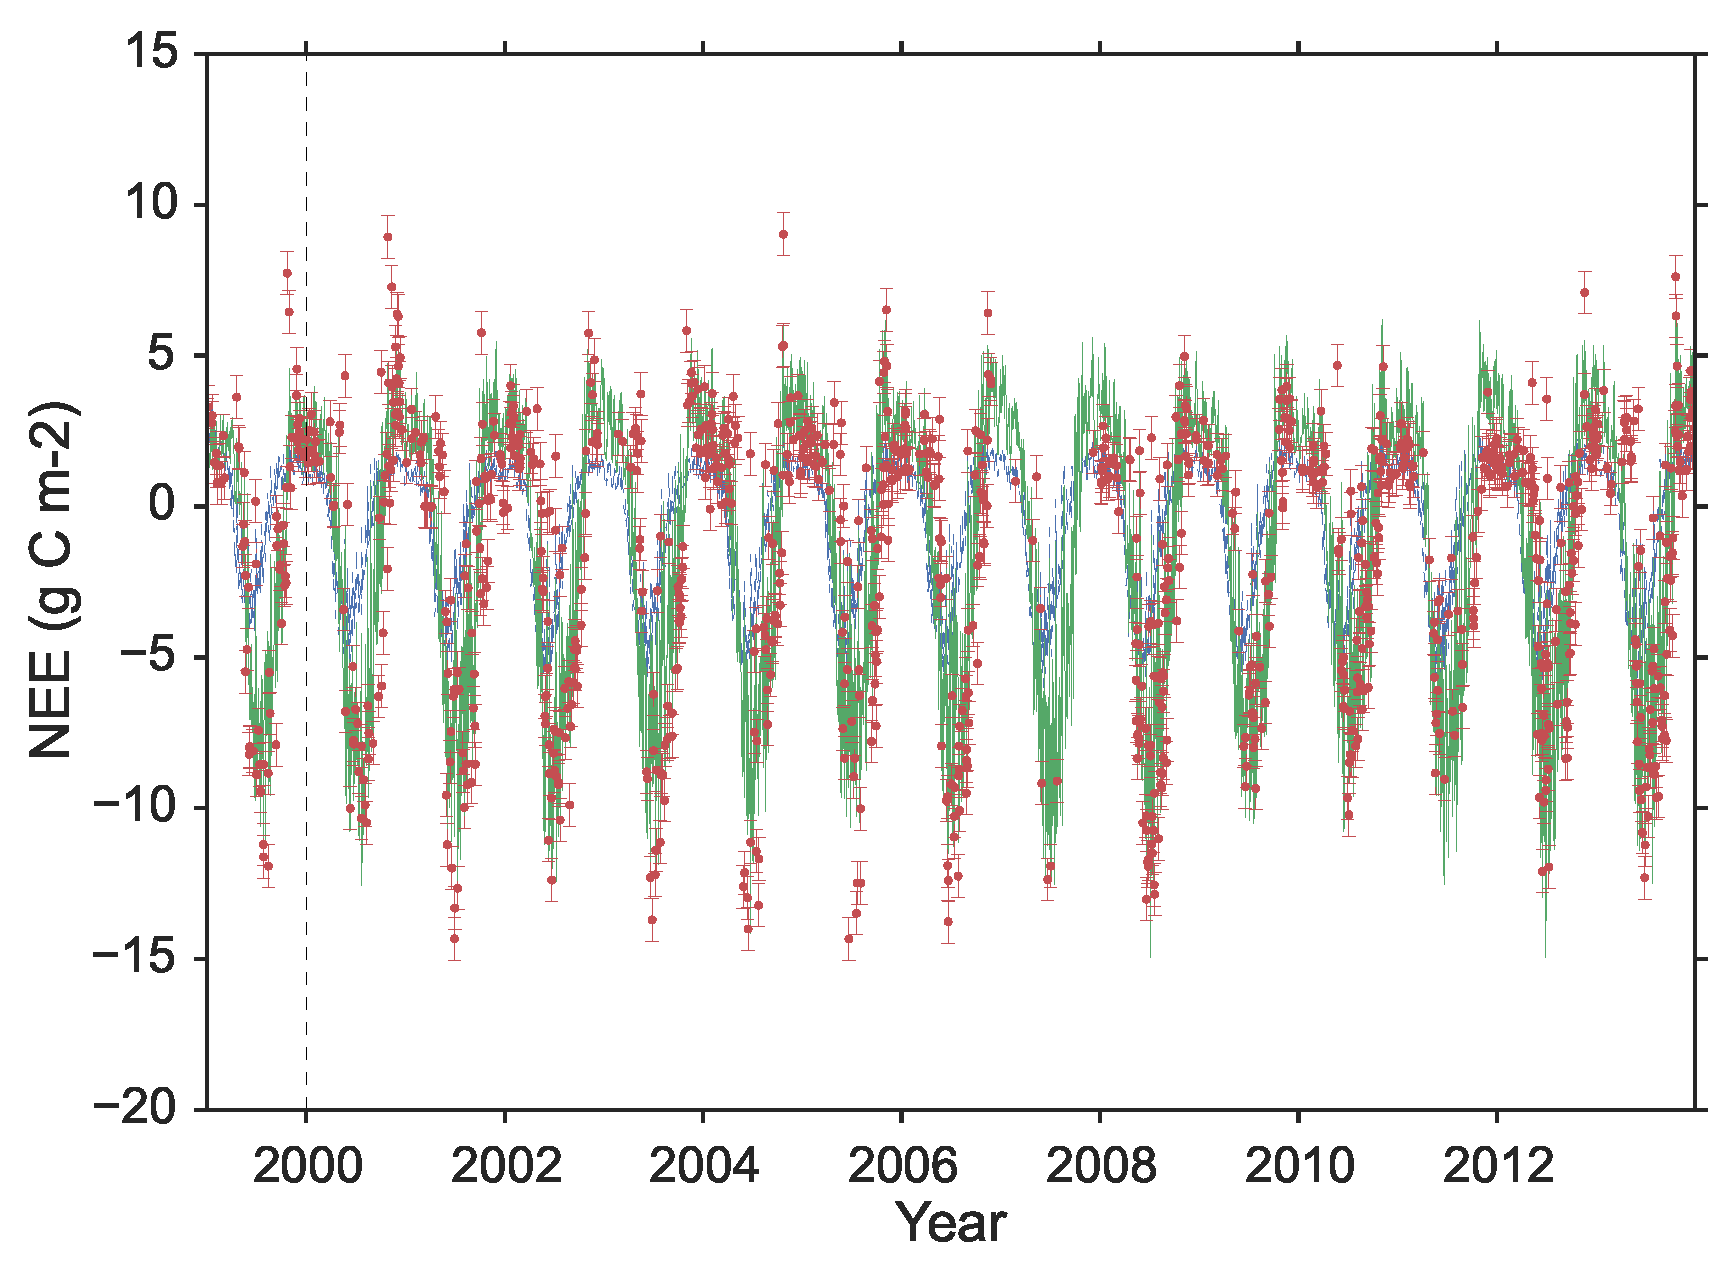
\includegraphics[width=\textwidth]{B4dvar.eps}
        \caption{Experiment B}
        \label{fig:4dvaredcBR}
    \end{subfigure}
    \begin{subfigure}[b]{0.49\textwidth}
        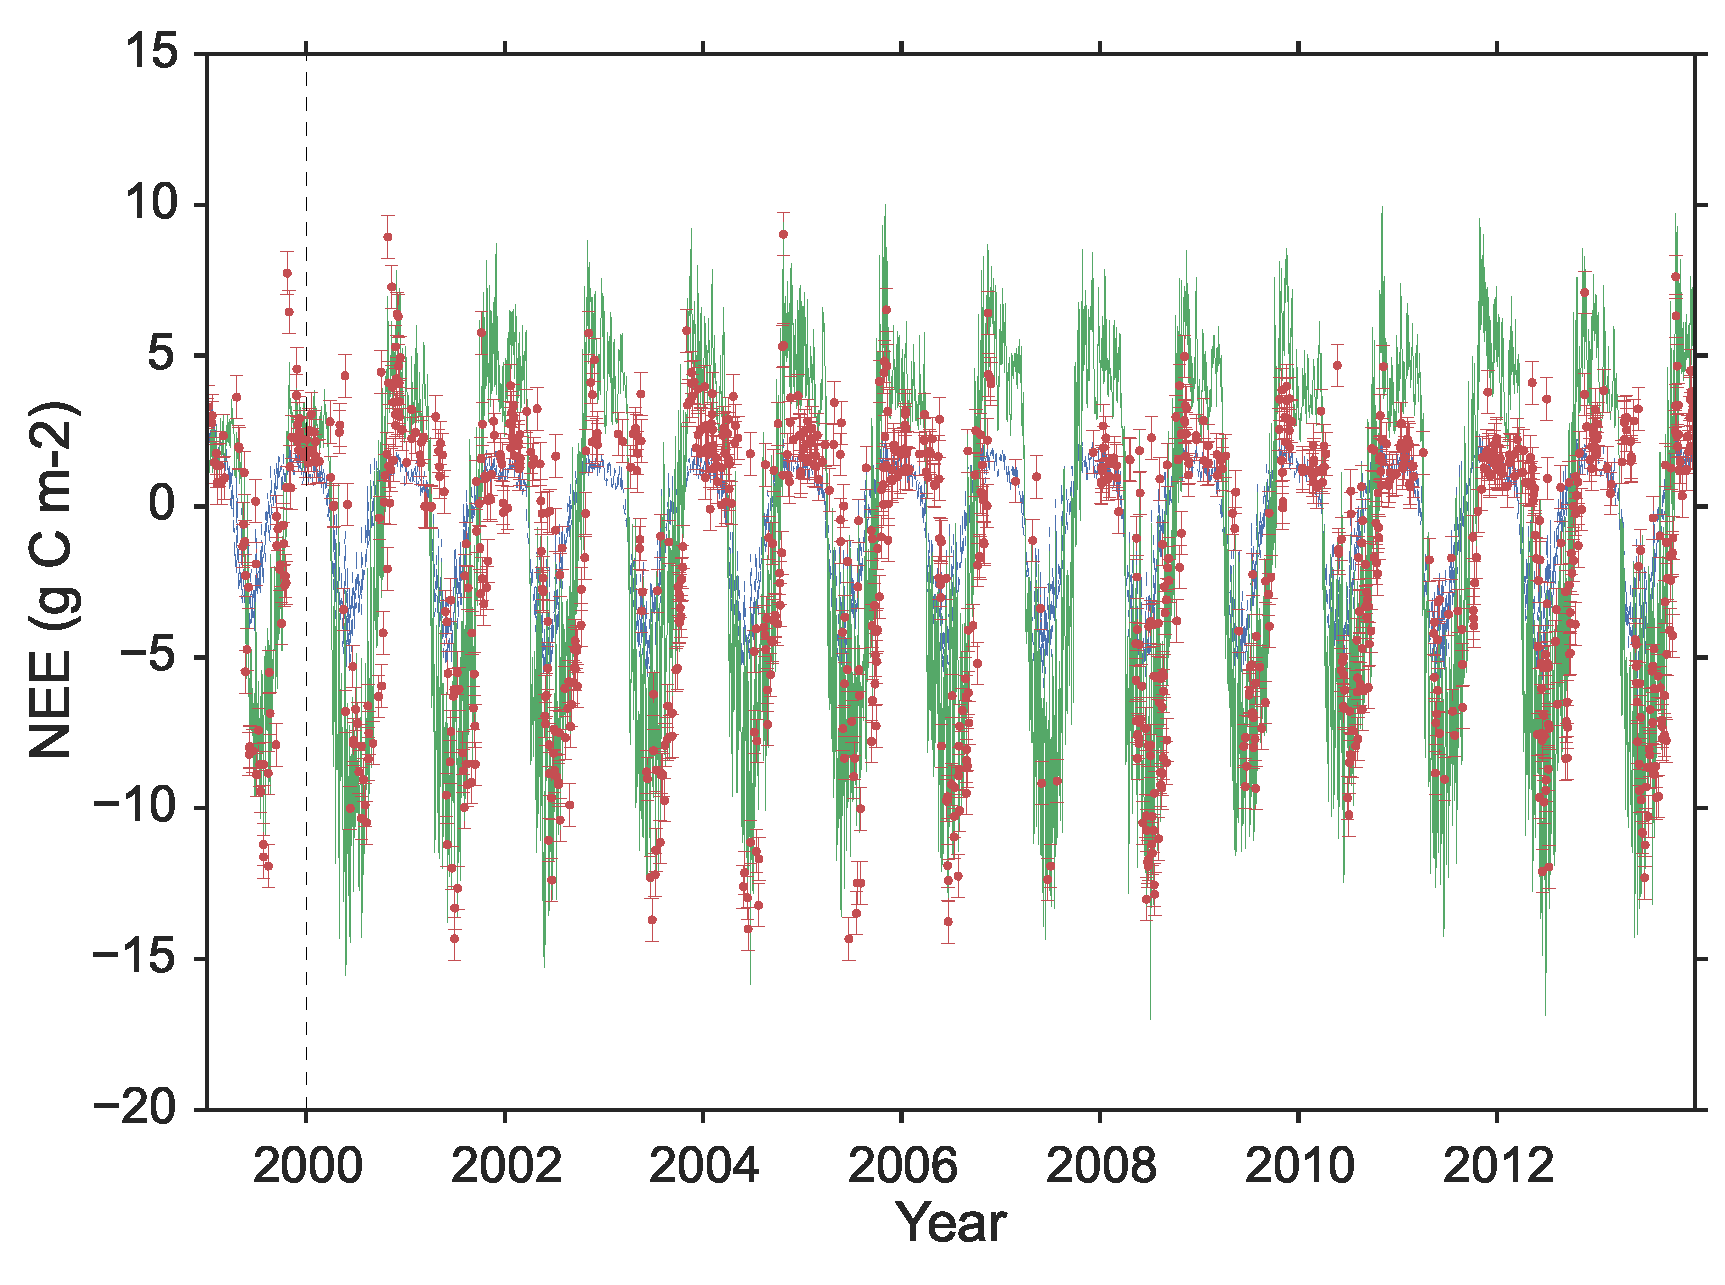
\includegraphics[width=\textwidth]{C4dvar.eps}
        \caption{Experiment C}
        \label{fig:4dvarBcorR}
    \end{subfigure}
    \begin{subfigure}[b]{0.49\textwidth}
        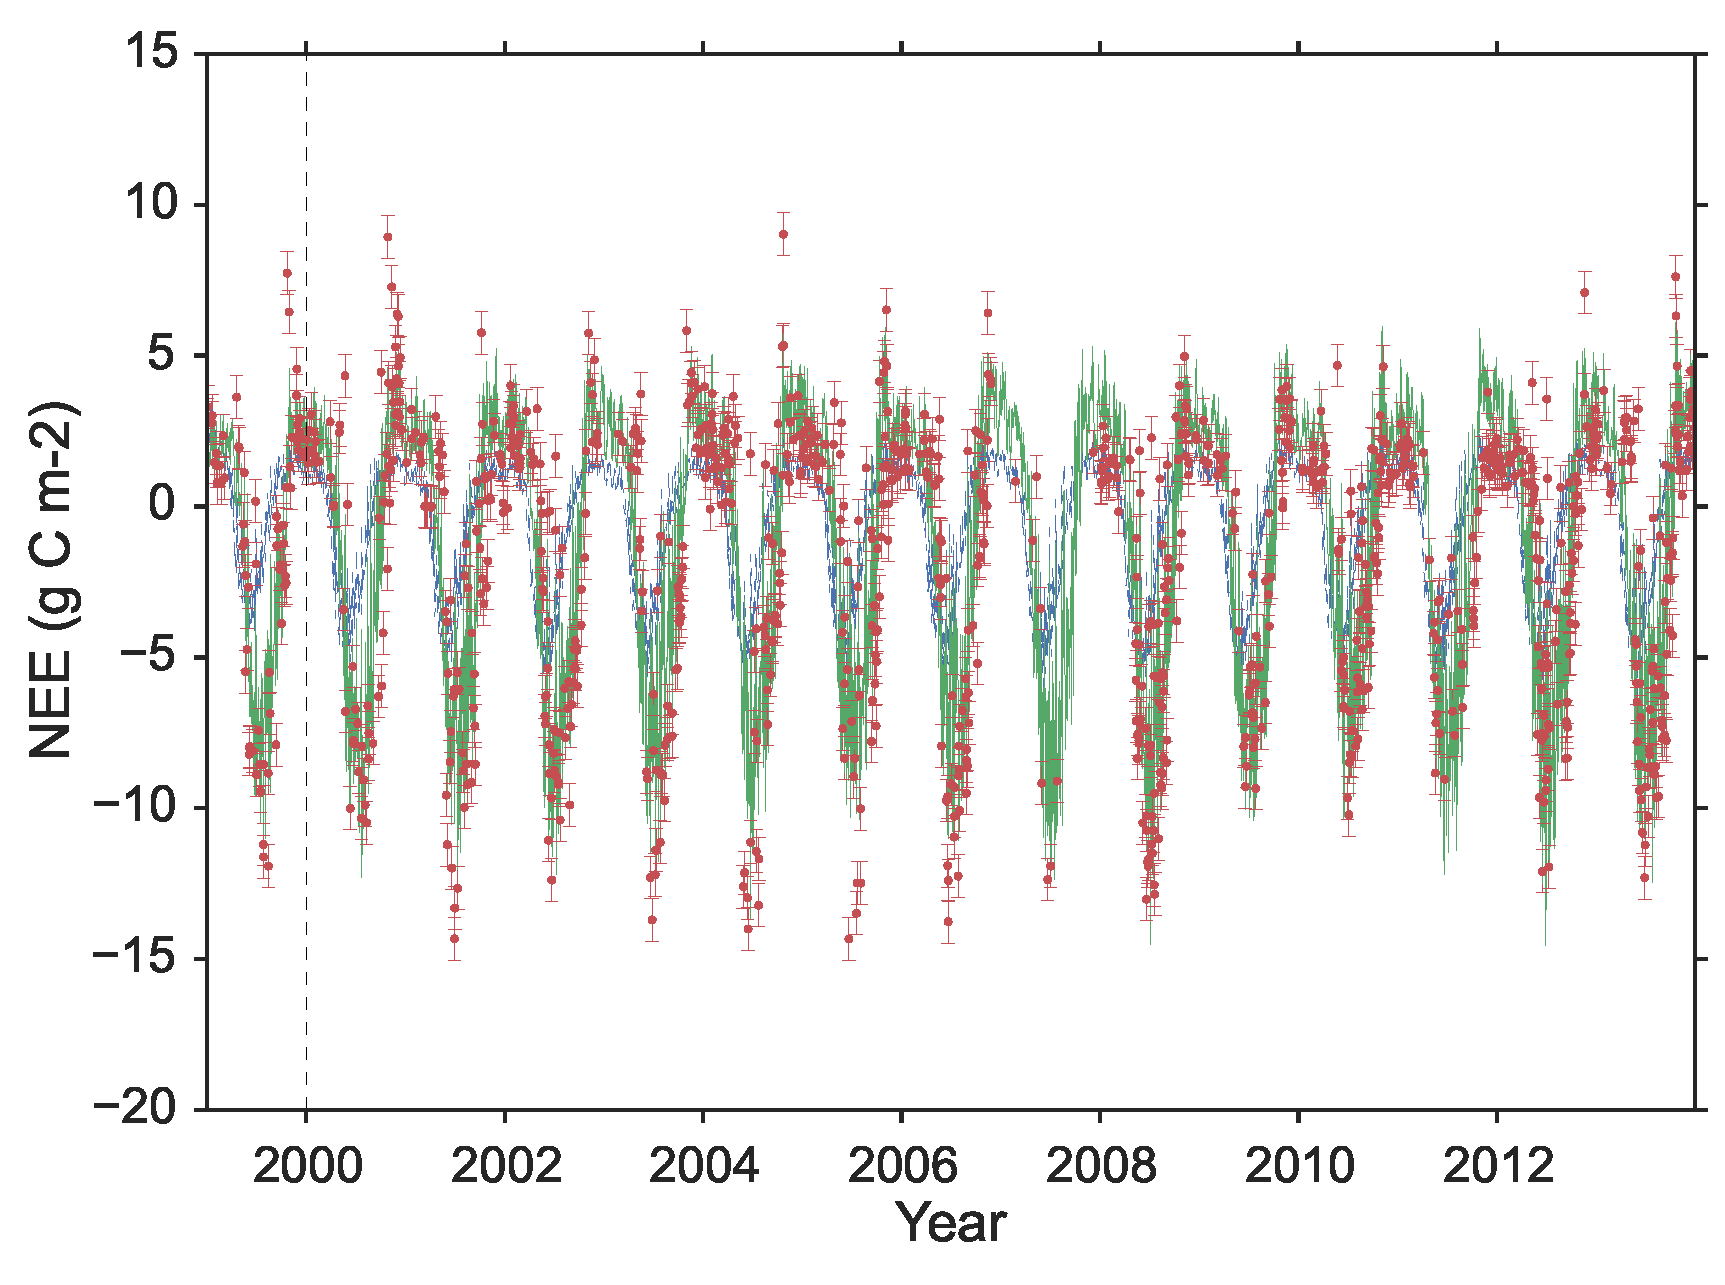
\includegraphics[width=\textwidth]{D4dvar.eps}
        \caption{Experiment D}
        \label{fig:4dvaredcBcorR}
    \end{subfigure}
    \caption{One year assimilation and fourteen year forecast of Alice Holt NEE with DALEC2, blue dotted line: background model trajectory, green line: analysis and forecast after assimilation, red dots: observations from Alice Holt flux site with error bars.}\label{fig:4dvar}
\end{figure}

\begin{figure}
    \centering
    \begin{subfigure}[b]{0.49\textwidth}
        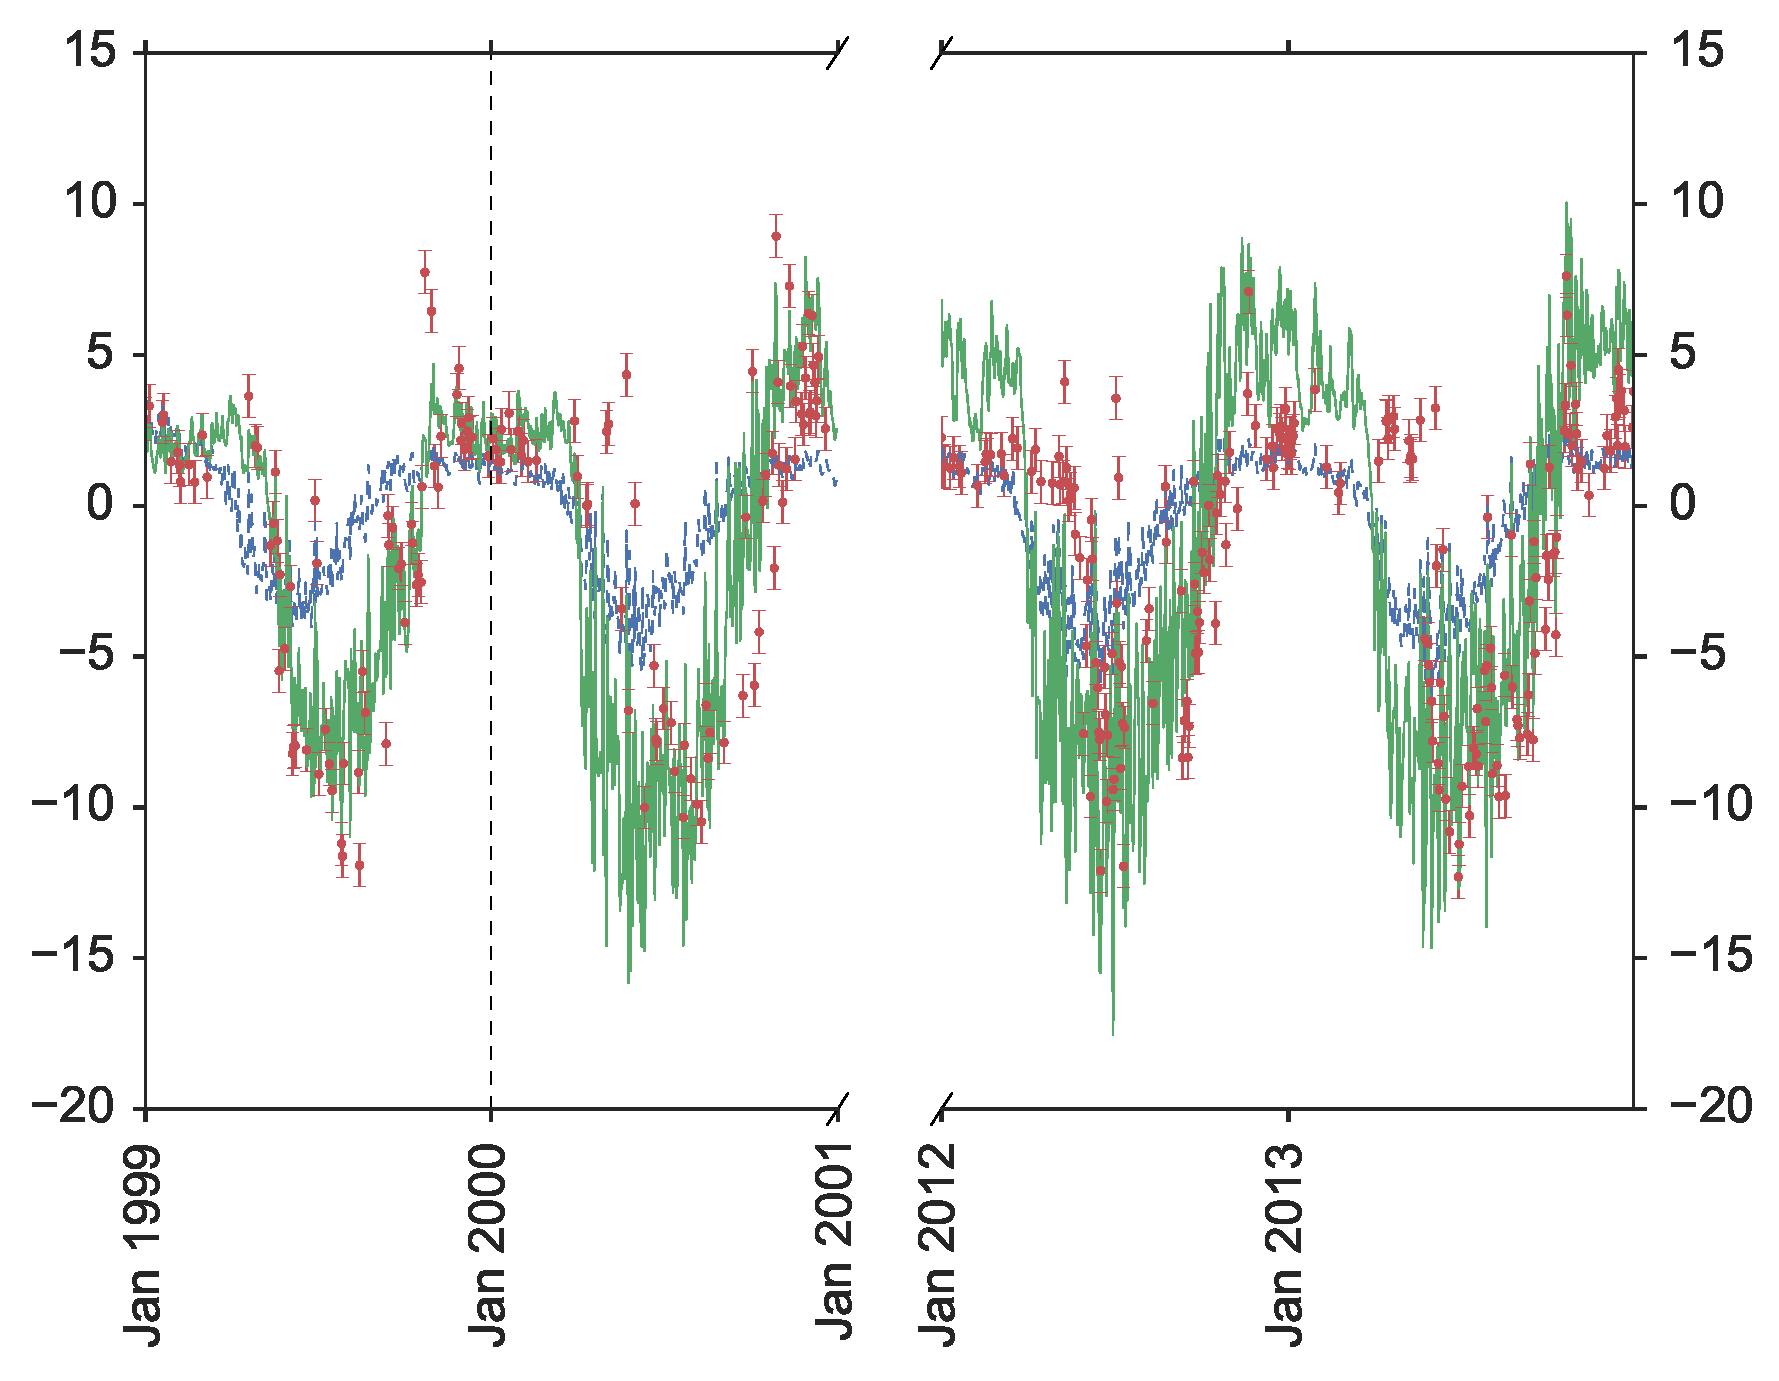
\includegraphics[width=\textwidth]{Abroke4dvar.eps}
        \caption{Experiment A}
        \label{fig:broke4dvardiagBR}
    \end{subfigure}
    \begin{subfigure}[b]{0.49\textwidth}
        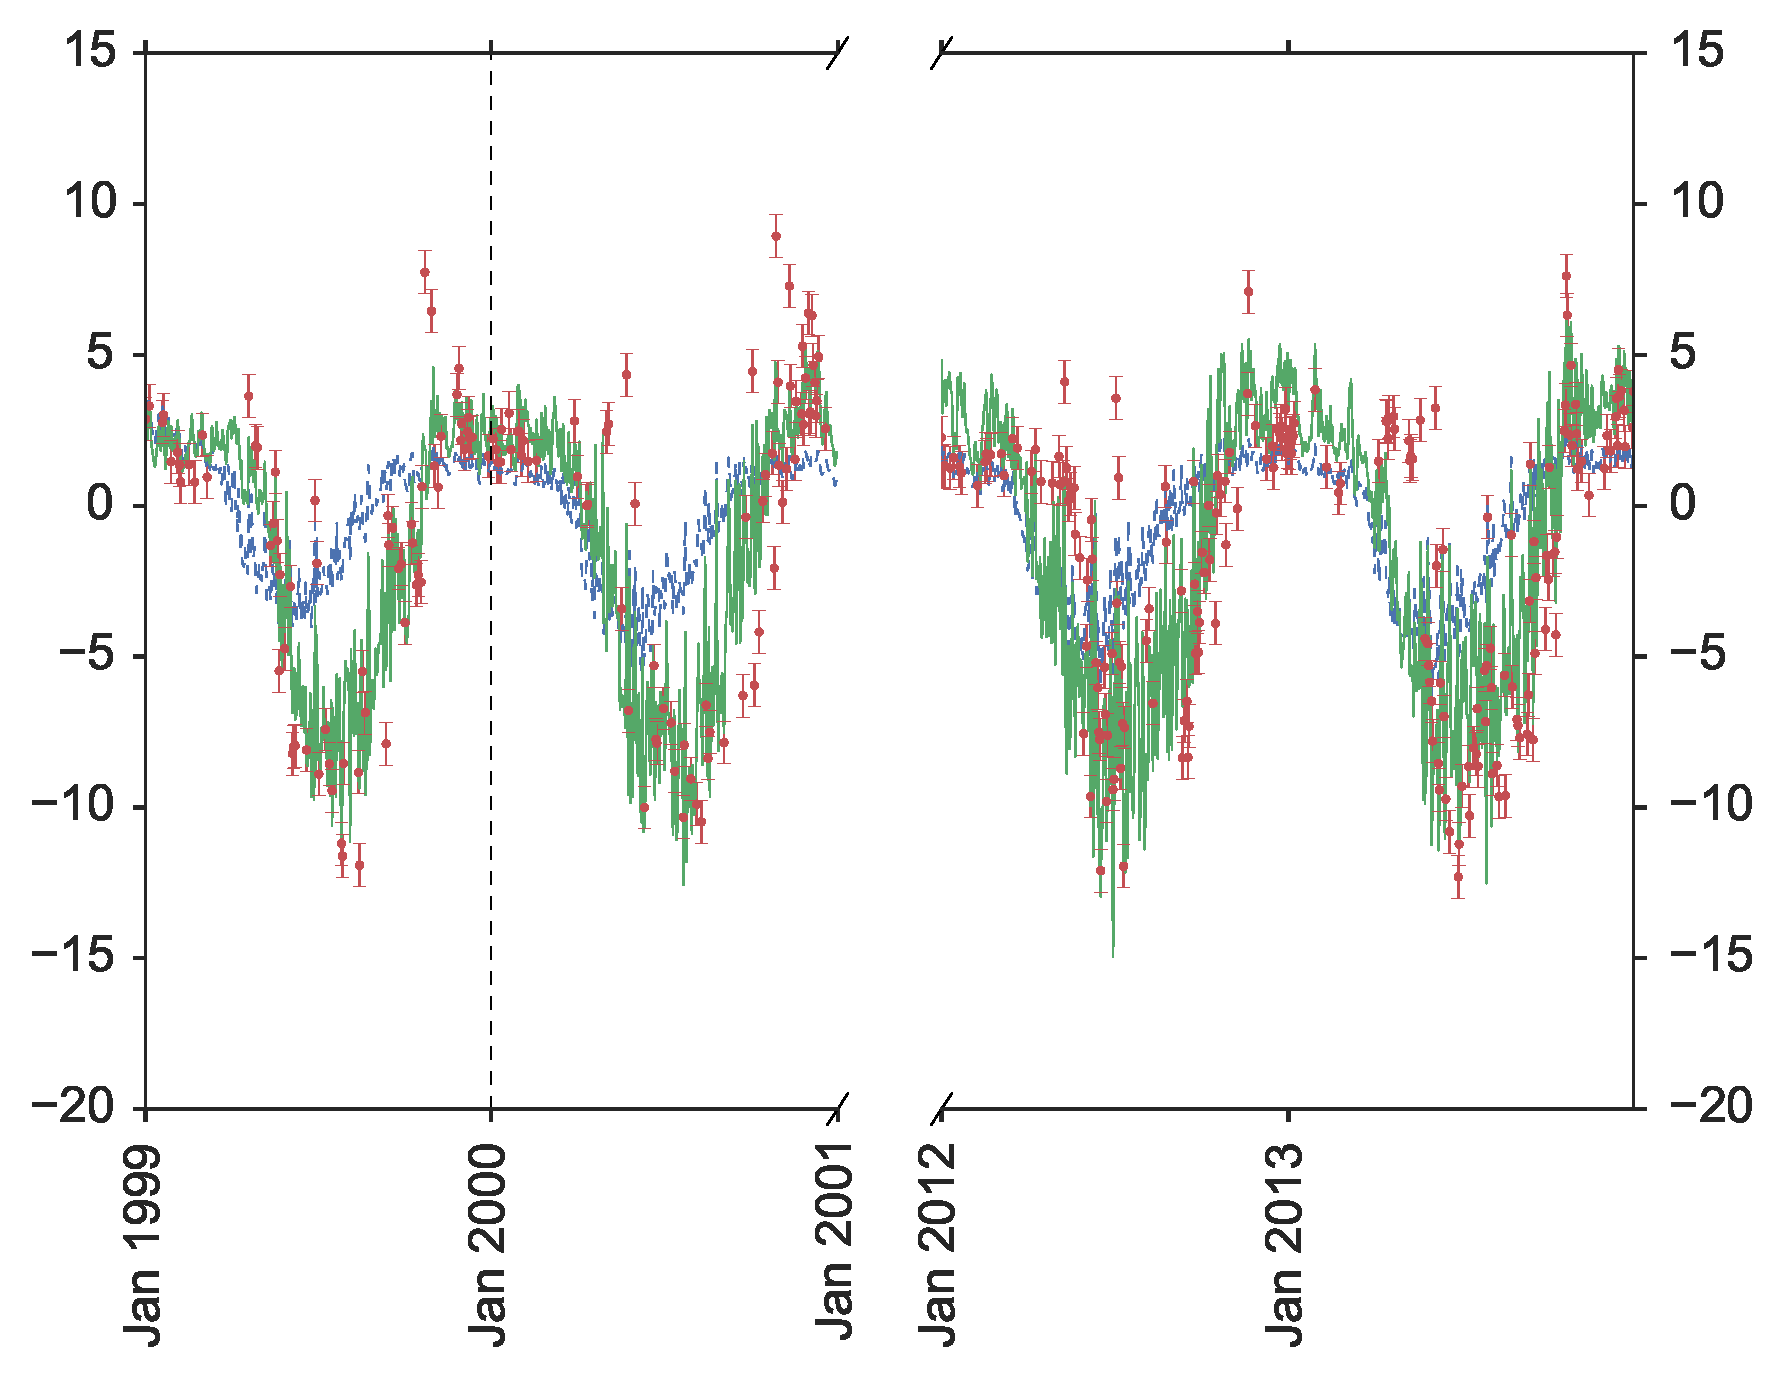
\includegraphics[width=\textwidth]{Bbroke4dvar.eps}
        \caption{Experiment B}
        \label{fig:broke4dvaredcBR}
    \end{subfigure}
    \begin{subfigure}[b]{0.49\textwidth}
        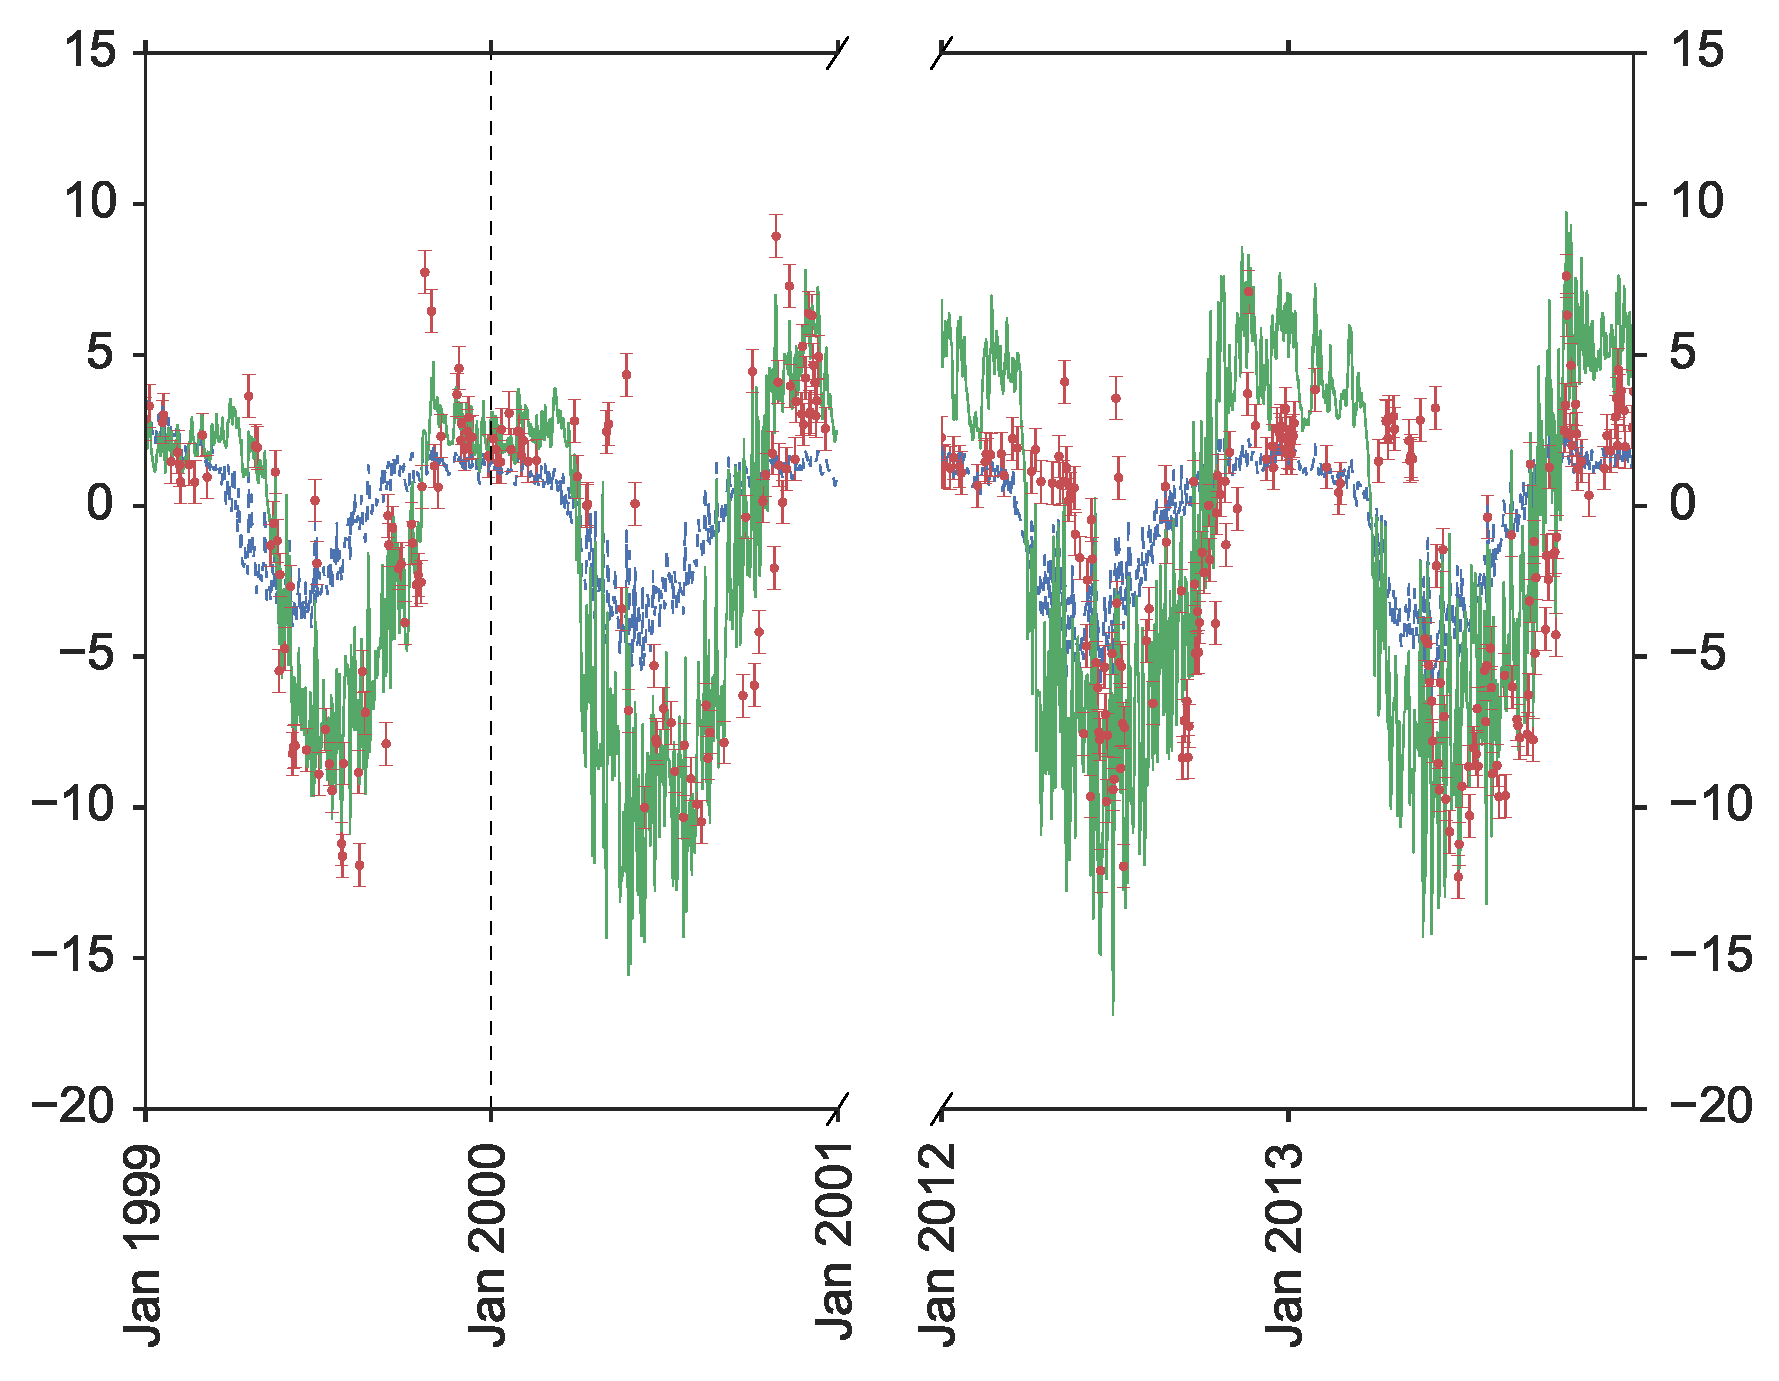
\includegraphics[width=\textwidth]{Cbroke4dvar.eps}
        \caption{Experiment C}
        \label{fig:broke4dvarBcorR}
    \end{subfigure}
    \begin{subfigure}[b]{0.49\textwidth}
        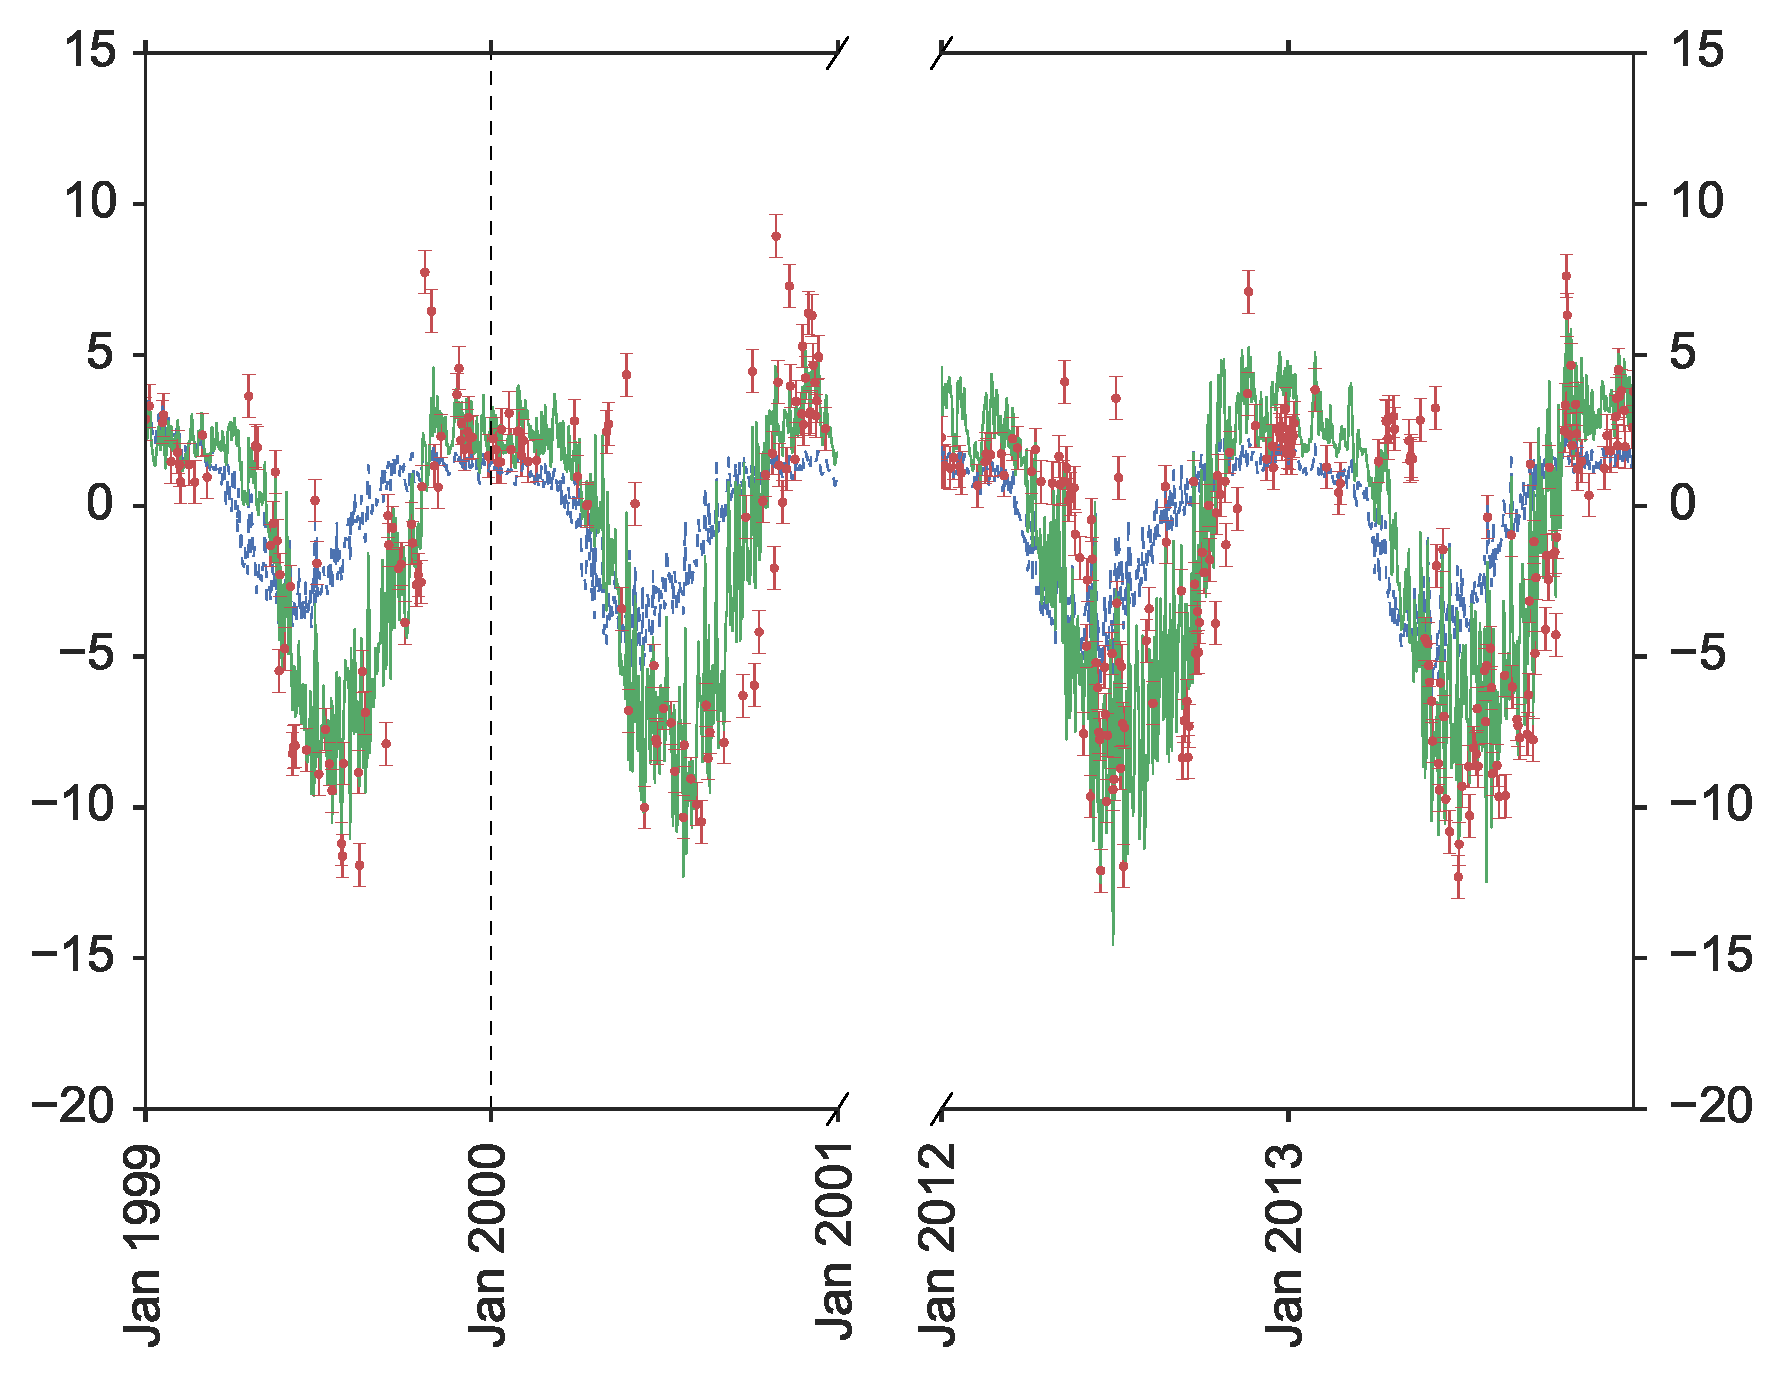
\includegraphics[width=\textwidth]{Dbroke4dvar.eps}
        \caption{Experiment D}
        \label{fig:broke4dvaredcBcorR}
    \end{subfigure}
    \caption{Broken plot showing the first and final two years results from the one year assimilation and fourteen year forecast of Alice Holt NEE with DALEC2, blue dotted line: background model trajectory, green line: analysis and forecast after assimilation, red dots: observations from Alice Holt flux site with error bars.}\label{fig:broke4dvar}
\end{figure}

\begin{figure}
    \centering
    \begin{subfigure}[b]{0.49\textwidth}
        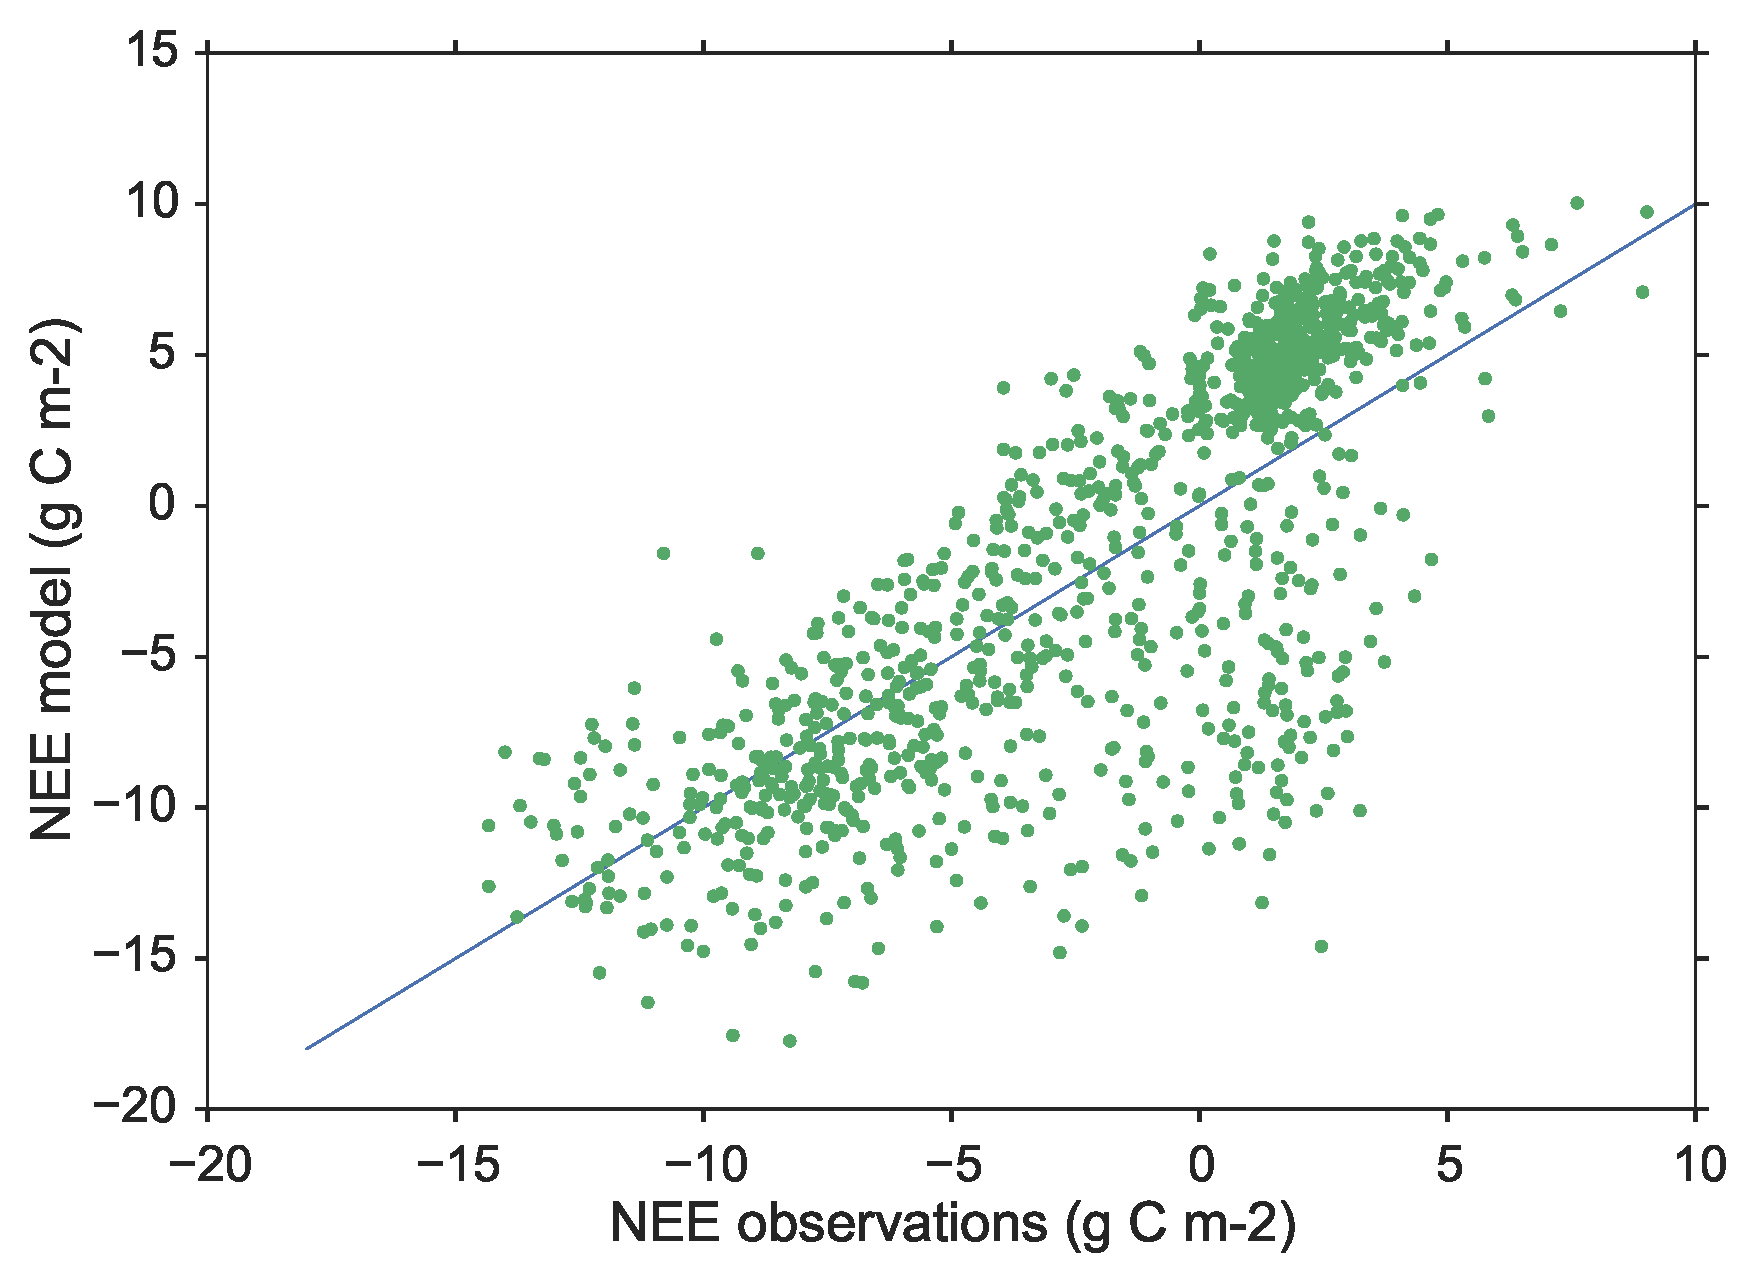
\includegraphics[width=\textwidth]{Afscat.eps}
        \caption{Experiment A}
        \label{fig:forecastscatBR}
    \end{subfigure}
    \begin{subfigure}[b]{0.49\textwidth}
        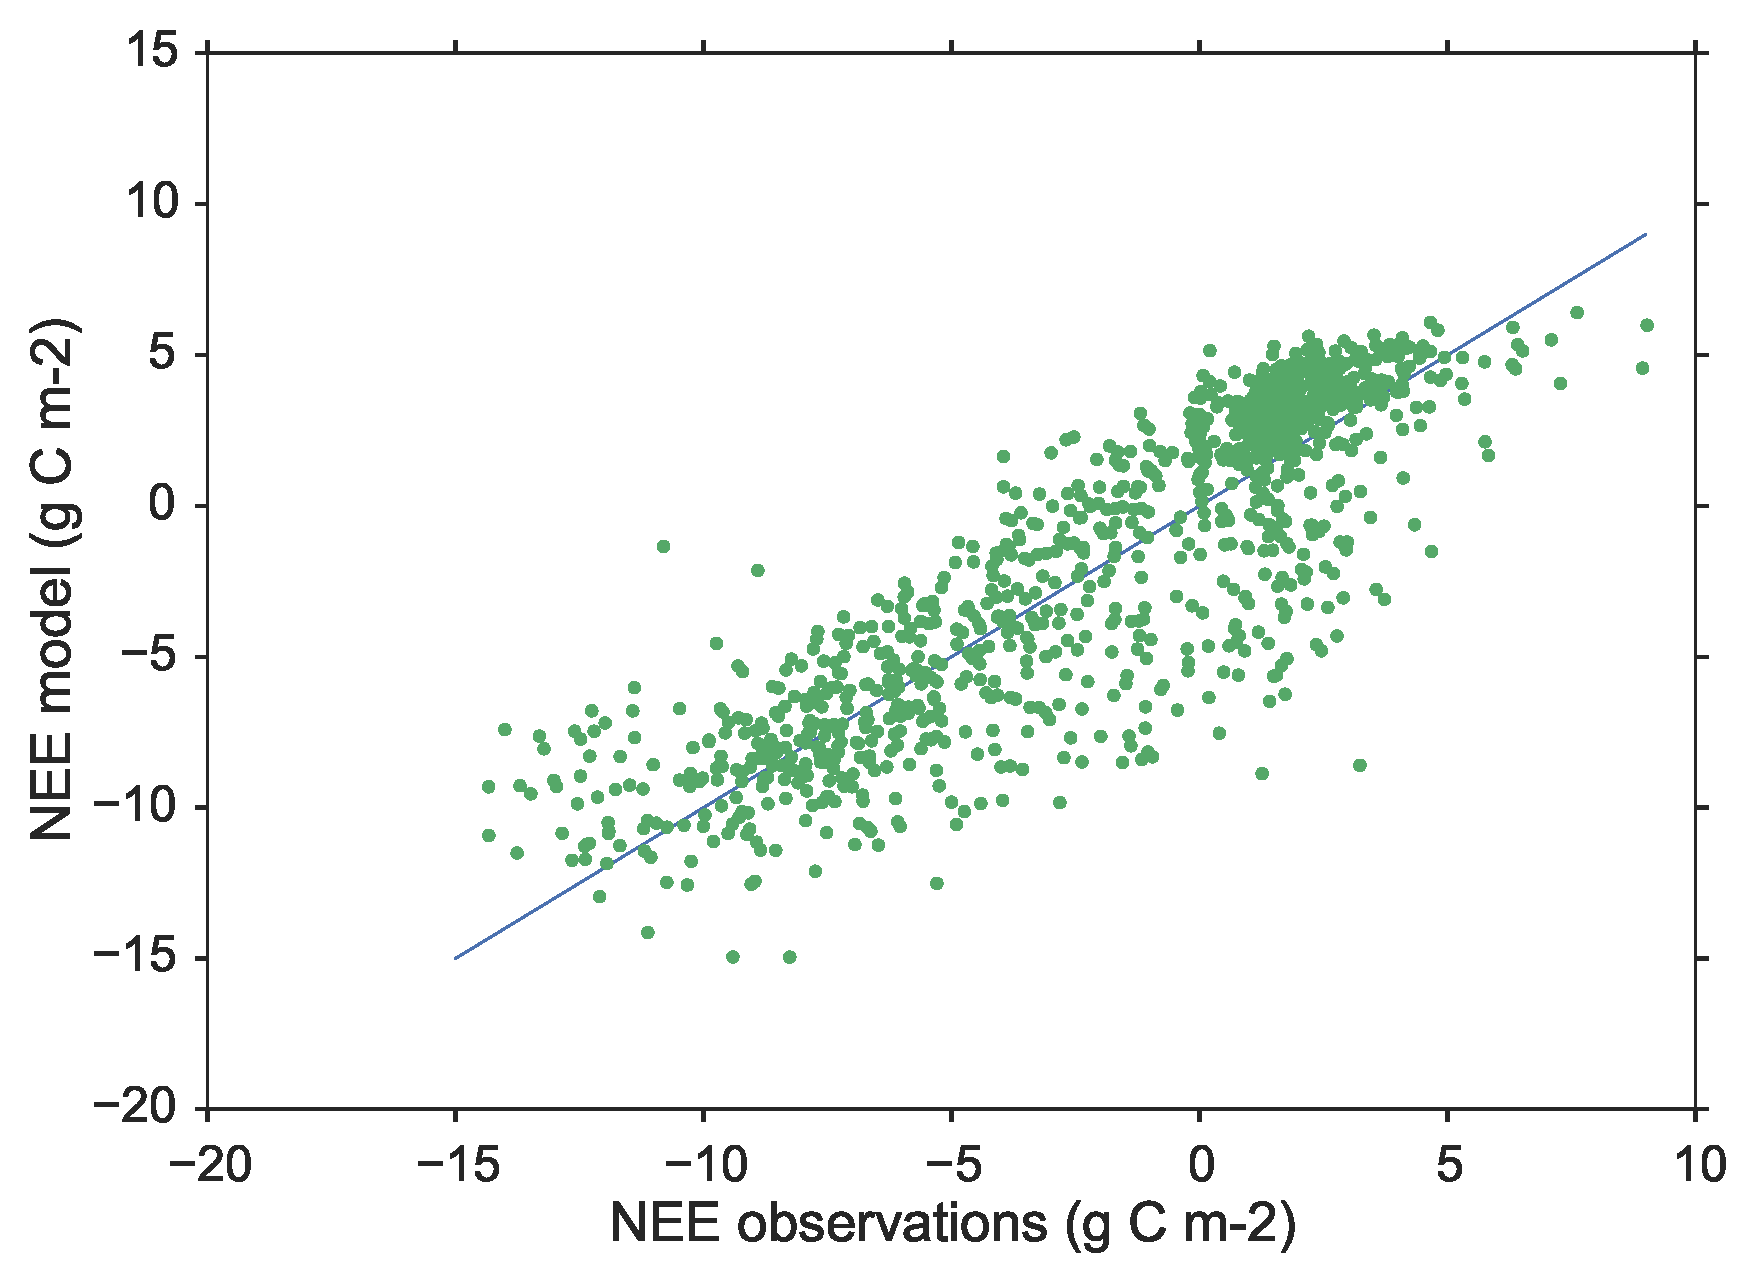
\includegraphics[width=\textwidth]{Bfscat.eps}
        \caption{Experiment B}
        \label{fig:forecastscatedcBR}
    \end{subfigure}
    \begin{subfigure}[b]{0.49\textwidth}
        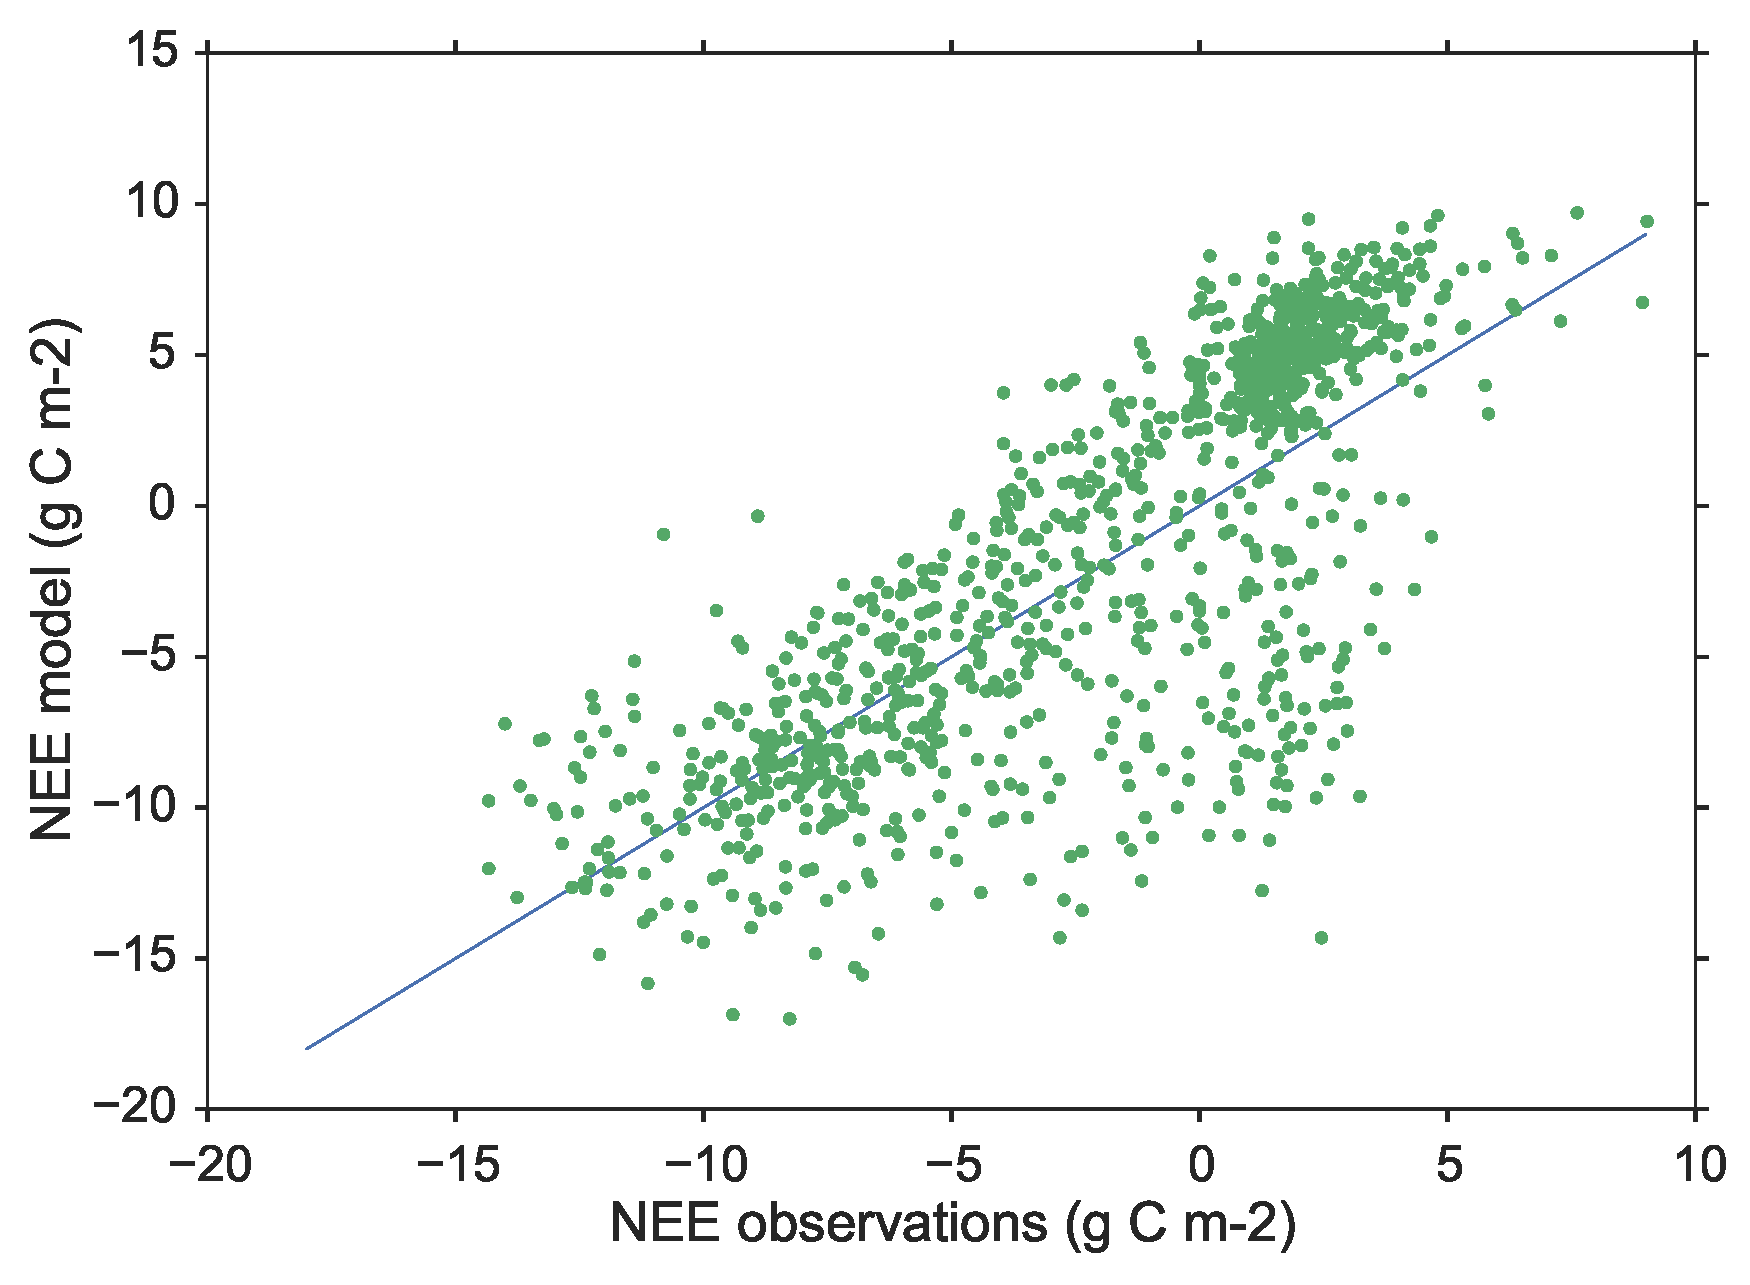
\includegraphics[width=\textwidth]{Cfscat.eps}
        \caption{Experiment C}
        \label{fig:forecastscatBcorR}
    \end{subfigure}
    \begin{subfigure}[b]{0.49\textwidth}
        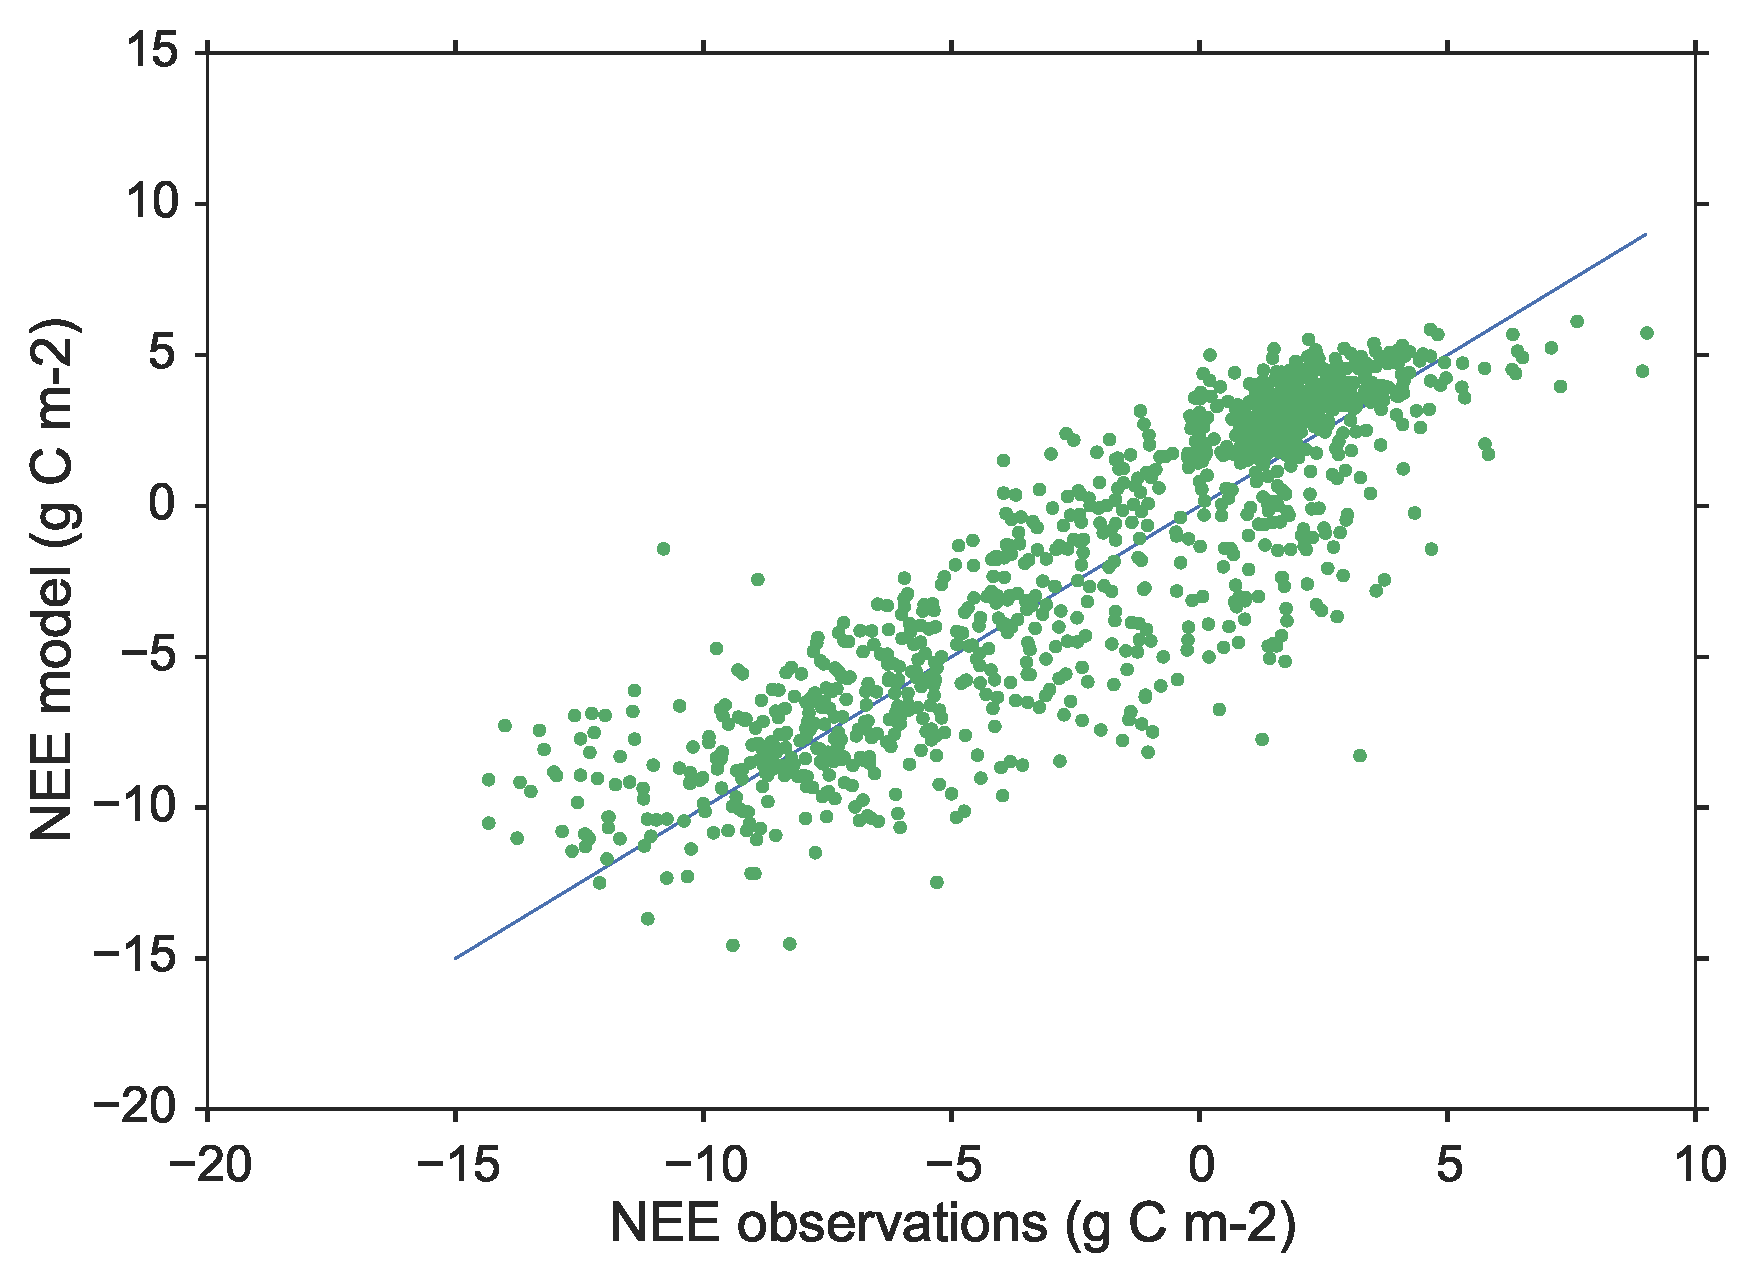
\includegraphics[width=\textwidth]{Dfscat.eps}
        \caption{Experiment D}
        \label{fig:forecastscatedcBcorR}
    \end{subfigure}
    \caption{Forecast scatter plot of modelled NEE vs. observations for 2000-2014 (green dots). Blue line represents the 1-1 line.}\label{fig:animals}
\end{figure}

\begin{figure}[ht]
    \centering
    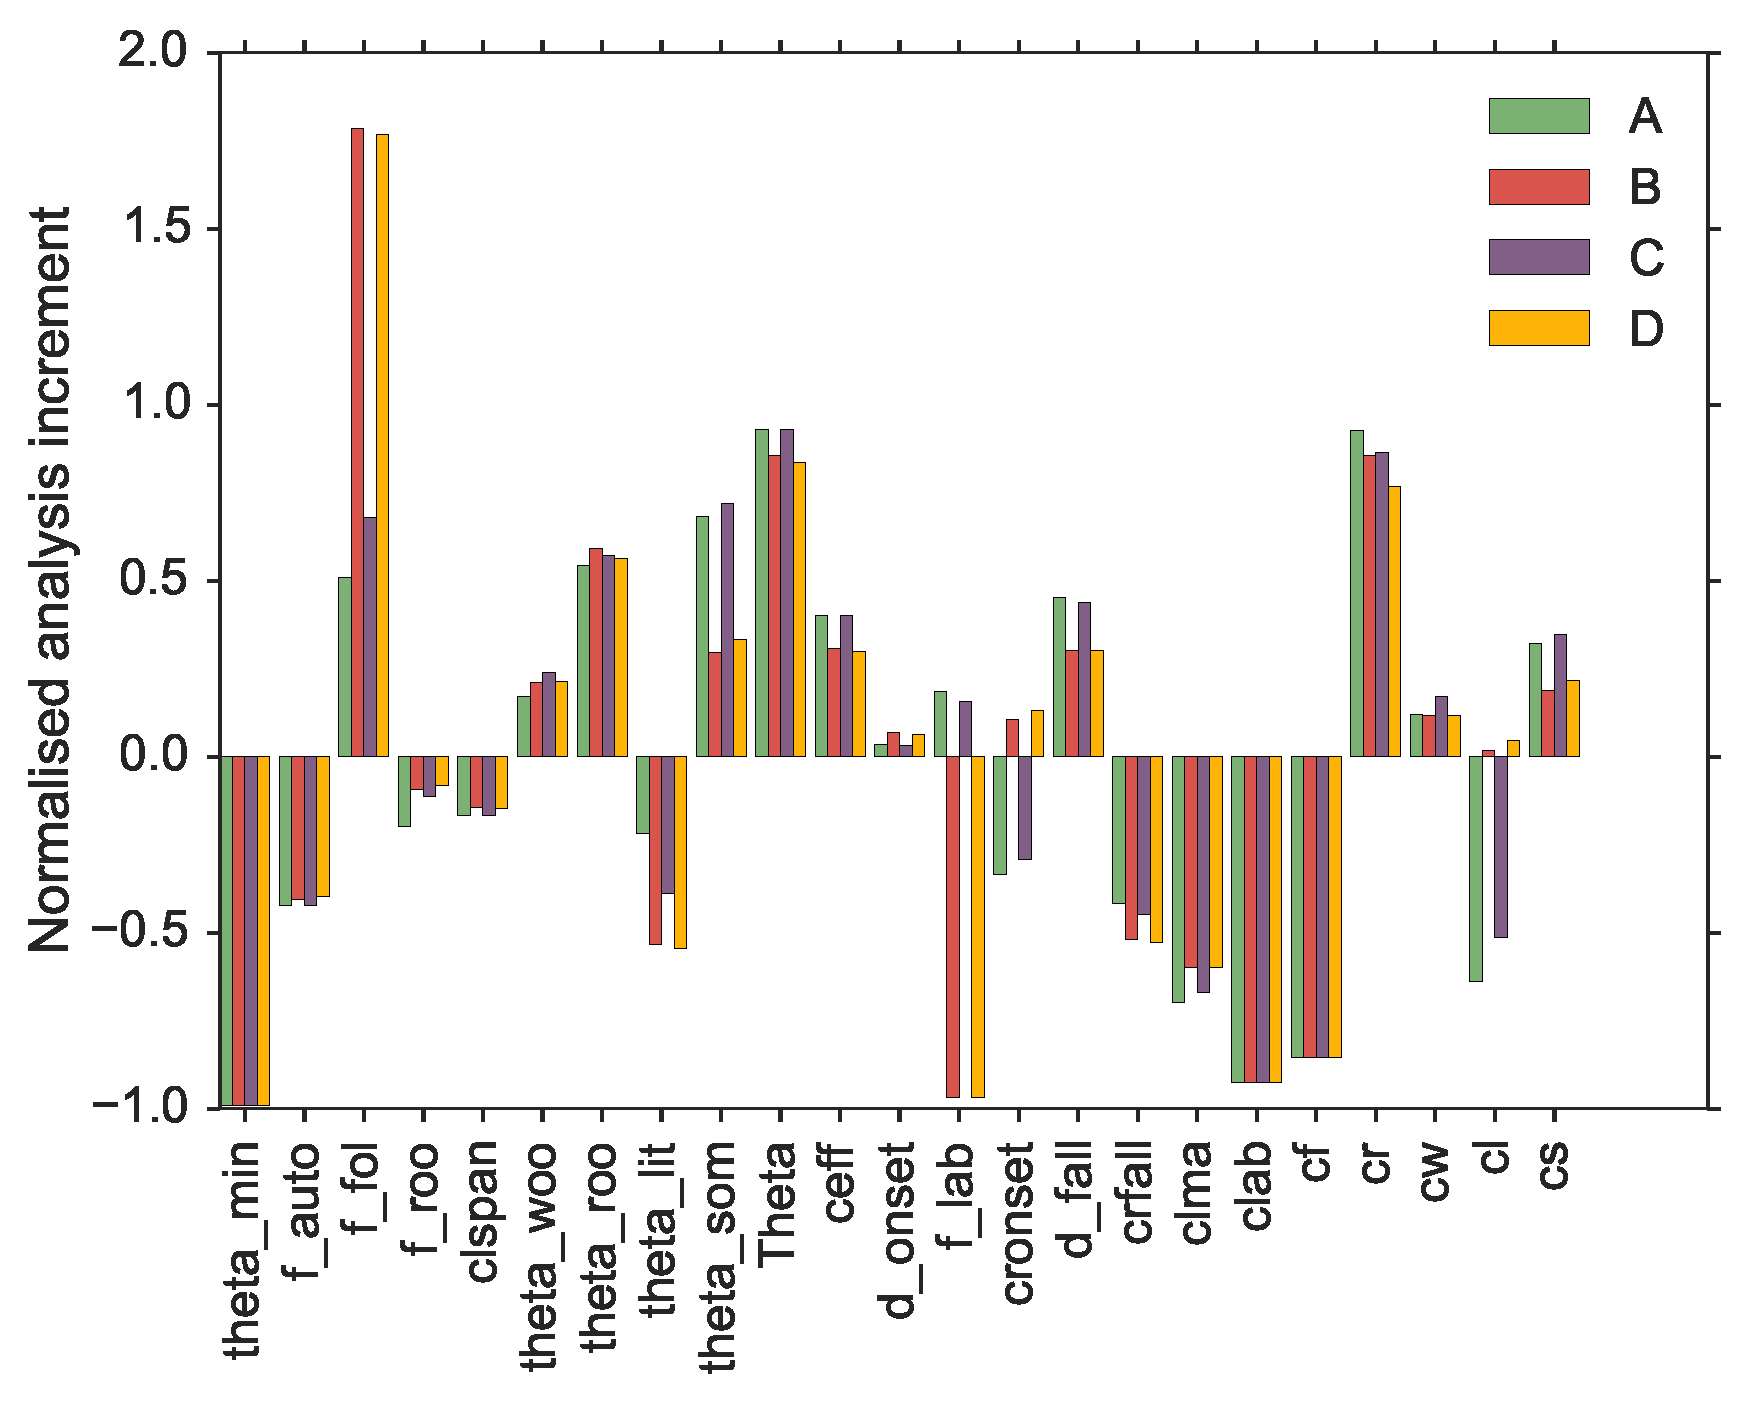
\includegraphics[width=0.5\textwidth]{inccvt.eps}
    \caption{Normalised analysis increment for the four experiments.}
    \label{fig:xa_inc}
\end{figure}

\subsection{Summary}

In our experiments we have shown that both $\textbf{B}_{corr}$ and $\hat{\textbf{R}}_{corr}$ have the effect of improving the model forecast of NEE. As it can be difficult to inspect the skill of a certain model by only plotting model trajectories, in figure~\ref{fig:taylordiag} we show Taylor diagrams displaying a statistical comparison of the four experiment and background analysis (1999-2000) and forecast (2000-2014) results with the observations of NEE. Here the radial distances from the origin to the points are proportional to the pattern standard deviations and the azimuthal positions give the correlation coefficient between the modelled and observed NEE \citep{Taylor2001}. If a model predicted the observations perfectly it would have a correlation coefficient of $1$ and a radial distance matching that of the observations (represented by the dotted line). Figure~\ref{fig:td_a} shows that all the experiments give very similar results in the analysis window (1999-2000) with all the experiment points closely grouped on top of each other. Whereas figure~\ref{fig:td_f} shows the significant difference between the experiment results in the forecast (2000-2014).

\begin{figure}[ht]
    \centering
    \begin{subfigure}[b]{0.49\textwidth}
        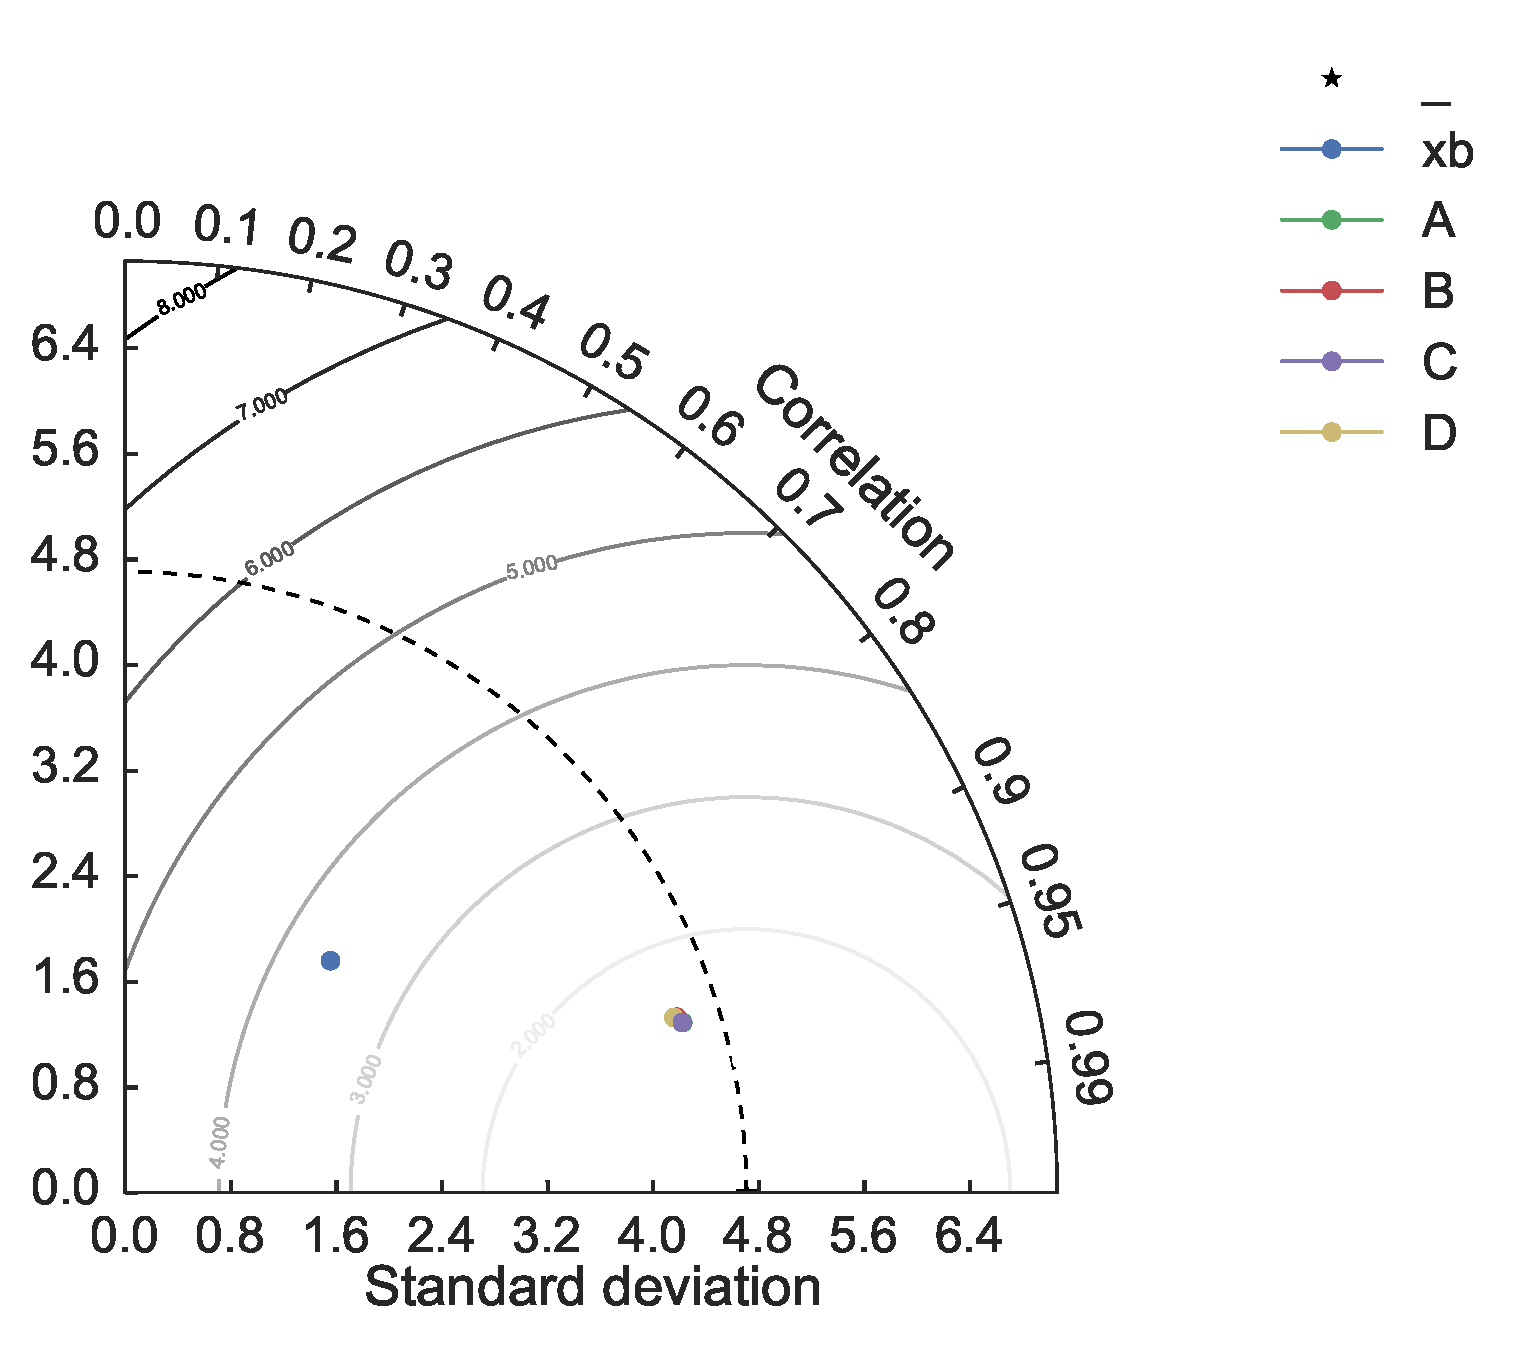
\includegraphics[width=\textwidth]{tdcvt_a.eps}
        \caption{Analysis (1999-2000)}
        \label{fig:td_a}
    \end{subfigure}
    \begin{subfigure}[b]{0.49\textwidth}
        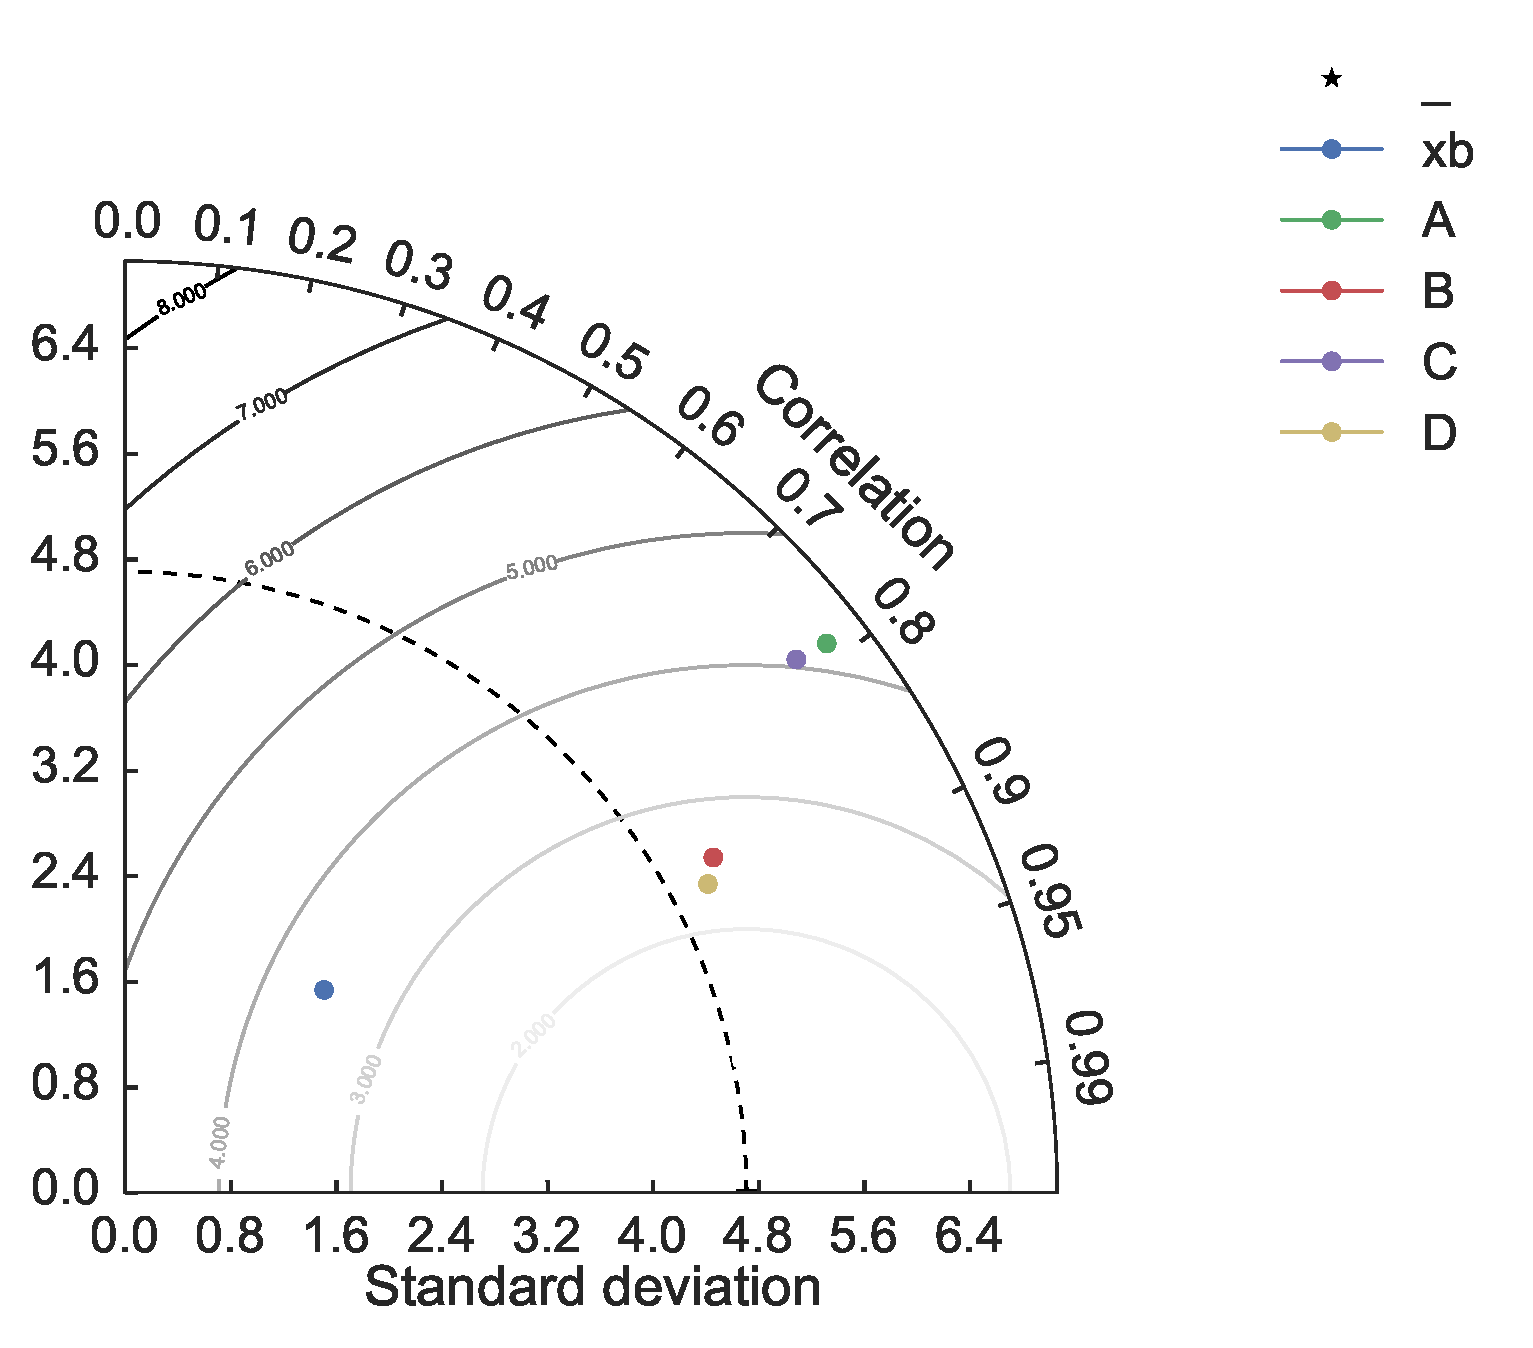
\includegraphics[width=\textwidth]{tdcvt_f.eps}
        \caption{Forecast (2000-2014)}
        \label{fig:td_f}
    \end{subfigure}
    \caption{Taylor diagrams displaying statistical comparison of the four experiment and background analysis (1999-2000) and forecast (2000-2014) results with observations of NEE $( \text{gCm}^{-2})$. The dotted line represents the standard deviation of the observations and the contours represent values of constant root mean square error between model and observations.}
    \label{fig:taylordiag}
\end{figure}

\begin{table}[ht] 
\begin{center}
	\begin{tabular}{| l | l | l | l |}
	\hline
	Experiment & RMSE $( \text{gCm}^{-2})$ & Bias $( \text{gCm}^{-2})$ & Correlation coefficient \\ \hline
	Background & $3.86$ & $-1.60$ & $0.70$ \\ \hline
	A & $1.36$ & $-0.03$ & $0.96$ \\ \hline
	B & $1.42$ & $-0.04$ & $0.95$ \\ \hline
	C & $1.37$ & $-0.09$ & $0.96$ \\ \hline
	D & $1.43$ & $-0.09$ & $0.95$ \\ 
	\hline
	\end{tabular}
	\caption{Analysis (1999-2000) results for experiments and background when judged against observed NEE.}
	\label{table:analysis_res}
\end{center} 
\end{table}

\begin{table}[ht] 
\begin{center}
	\begin{tabular}{| l | l | l | l |}
	\hline
	Experiment & RMSE $( \text{gCm}^{-2})$ & Bias $( \text{gCm}^{-2})$ &  Correlation coefficient \\ \hline
	Background & $3.86$ & $-1.36$ & $0.66$ \\ \hline
	A & $4.22$ & $-0.30$ & $0.79$ \\ \hline
	B & $2.56$ & $-0.20$ & $0.87$ \\ \hline
	C & $4.09$ & $-0.51$ & $0.78$ \\ \hline
	D & $2.38$ & $-0.33$ & $0.88$ \\ 
	\hline
	\end{tabular}
	\caption{Forecast (2000-2014) results for experiments and background when judged against observed NEE.}
	\label{table:forecast_res}
\end{center} 
\end{table}


\section{Discussion}


In this paper we have implemented the DALEC2 functional ecology model in a 4D-Var data assimilation scheme, building an adjoint of the DALEC2 model and applying rigorous tests to our scheme. Using 4D-Var can provide much faster assimilation results than MCMC techniques as we have knowledge of the derivative of the model. For our experiments the 4D-Var routine has taken $O(10^{2})$ function evaluations to converge to a minimum, whereas MCMC techniques using the same model take $O(10^{8})$ function evaluations \citep{Bloom2015}. However we do also assume that the problem is Gaussian whereas MCMC techniques do not. We have shown that 4D-Var is a valid tool for improving the DALEC2 model estimate of NEE and that even when assimilating only a single year of NEE observations we can improve our forecast significantly. In practice this type of data assimilation routine would be run in cycling mode running the analysis from the first year as the background for the second then iterating this until all data is assimilated.

We then considered the nature of background and observational errors. The effect of specifying parameter-state correlations in our background information and serial correlations between our observation errors was explored.

The technique presented here to specify ${\mathbf{B}}_{corr}$ has been shown to significantly improve forecasts of NEE over using a diagonal representation of ${\mathbf{B}}$. These results agree with those of \citet{smith2009variational} where the importance of specifying parameter-state correlations when performing joint parameter-state estimation with variational data assimilation is shown. The method for specifying ${\mathbf{B}}_{corr}$ in this paper used a series of ecological dynamical constraints taken from \citet{Bloom2015}. In cases where these type of constraints are not available there are other methods to build correlations into $\textbf{B}$. One technique we also tested (not presented here) to create a correlated $\textbf{B}$ involved evolving an ensemble of state vectors over the length of the chosen assimilation window using the model (DALEC2) and then taking the covariance of the evolved ensemble. This gave us a \textbf{B} with parameter-state and state-state correlations, but no parameter-parameter correlations as the parameters are not updated by the model. Using the $\textbf{B}$ created with this method also improved assimilation results significantly over using a diagonal $\textbf{B}$. Many different tests were run using different background vectors and variances and it was found that specifying some form of correlation structure in $\textbf{B}$ always made some improvement to the results of our assimilation. As this work has only considered a single site more work is required to investigate the effect of including correlations in background information at sites with different types of vegetation. 

In NWP it has been shown that including correlations in $\textbf{R}$ can help improve data assimilation results \citep{weston2014accounting}. However the specified correlations have most commonly been spatial correlations with observations errors still being considered independent in time. In this paper we have shown that including correlations between observation errors in time can also improve data assimilation results, here improving the DALEC2 model forecast of NEE. We expect including these serial correlations to have an even greater impact when assimilating more than one data stream. When assimilating multiple data streams more frequently sampled observation types (such as NEE) have much more impact on the assimilation than data streams sampled less frequently. Specifying serial correlations between observations of the same type has the effect of reducing the weight given to the mean of the observations \citep{jarvinen1999variational}, thus allowing less frequent data streams to have more impact on the assimilation. Using the form of $\hat{\mathbf{R}}$ given in this paper for specifying serial correlations will also allow us to specify serial correlations between different observation types. When running the model with a day-night time step this will allow us to build in the type of correlations investigated by \citet{Baldocchi2015} between ecosystem respiration and canopy photosynthesis. More work is needed to investigate the effect of including correlations between observations error statistics when assimilating multiple data streams.

The $\hat{\mathbf{R}}_{corr}$ presented in this paper has a weak correlation ($a=0.3$) between observations of NEE in time, this representation of $\hat{\mathbf{R}}_{corr}$ has improved the model forecast of NEE. However other choices of $\hat{\mathbf{R}}_{corr}$ (with stronger correlations between observations) tested for this paper degraded the forecast. This is probably due to the specified correlations being unrealistic and suggests a more diagnostic approach is needed for the calculation of serial correlations in $\hat{\mathbf{R}}$. One option would be to adapt the \citet{desroziers2005diagnosis} diagnostic, which has been used successfully in NWP for diagnosing observation error correlations for observations taken at the same time, and extending this technique to diagnose serial correlations. This will form the basis of future work.

Including correlations in both $\textbf{B}$ and $\textbf{R}$ improve the DALEC2 model forecast of NEE significantly. From the results in experiment D (using both $\textbf{B}_{corr}$ and $\hat{\textbf{R}}_{corr}$) and integrating over the area of the Alice Holt flux site ($\sim 0.93\text{km}^2$) the forecasted (2000-2014) total carbon uptake for the Alice Holt research site is $5.04\times 10^9 \text{gC}$. In comparison the less accurate results from experiment A (using $\textbf{B}_{diag}$ and $\hat{\textbf{R}}_{diag}$) predict a total carbon uptake of $5.26 \times 10^9\text{gC}$, a difference of $2.25 \times 10^8\text{gC}$. This is quite a substantial difference as we are considering the carbon uptake of a small ($\sim 0.93\text{km}^2$) research site only.

\section{Conclusion}

Largely functional ecology and land surface model data assimilation routines treat prior estimates of parameter and state uncertainties and observation error statistics as independent and uncorrelated. In this paper we have shown the importance of including estimates to such correlations, especially between background parameter and state error statistics when performing joint parameter-state estimation.

When performing joint parameter-state estimation including correlations in the background error covariance matrix significantly improves our forecast after assimilation, in comparison to using a diagonal representation of $\textbf{B}$. Specifying serial correlations between observation errors in $\hat{\textbf{R}}$ also improves our forecast and we expect these correlations to have a greater impact when assimilating more than one data stream. More work is needed to investigate the effect of including these correlations at different sites and when assimilating multiple data streams. The development of a more diagnostic tool for the calculation of the error correlation structure in $\hat{\textbf{R}}$ is also important.  

When including both parameter-state correlations in $\textbf{B}$ and time correlations between observation errors in $\hat{\textbf{R}}$ and assimilating only a single year of NEE observations we can forecast 14 years of NEE observations with a root-mean square error of $2.38\text{gCm}^{-2}\text{day}^{-1}$ and a correlations coefficient of $0.88$. This is a significant reduction in error from the results when using a $\textbf{B}$ and $\hat{\textbf{R}}$ with no specified correlations of $4.22\text{gCm}^{-2}\text{day}^{-1}$ and a correlation coefficient of $0.79$.

\section{Acknowledgements}
Luke, FR, NERC, NCEO, ({\color{red}Which are needed? How to do this?})

\bibliography{../PhD}{}
%\bibliographystyle{plain}

\section*{Appendix}

\begin{table}[ht] 
\begin{center}
	\begin{tabular}{| l | l | l | l |}
	\hline
	Parameter & Description & Background & \pbox{7cm}{Standard \\deviation} \\ \hline
$\theta_{min}$ & Litter mineralisation rate (day$^{-1}$) & $9.810e-04$ & $2.030e-03$ \\ \hline
$f_{auto}$ & Autotrophic respiration fraction & $5.190e-01$ & $1.168e-01$  \\ \hline
$f_{fol}$ & Fraction of GPP allocated to foliage & $1.086e-01$ & $1.116e-01$ \\ \hline
$f_{roo}$ & Fraction of GPP allocated to fine roots & $4.844e-01$ & $2.989e-01$ \\ \hline
$c_{lspan}$ & Determines annual leaf loss fraction & $1.200e+00$ & $1.161e-01$  \\ \hline
$\theta_{woo}$ & Woody carbon turnover rate (day$^{-1}$) & $1.013e-04$ & $1.365e-04$  \\ \hline
$\theta_{roo}$ & Fine root carbon turnover rate (day$^{-1}$) & $3.225e-03$ & $2.930e-03$ \\ \hline
$\theta_{lit}$ & Litter carbon turnover rate (day$^{-1}$) & $3.442e-03$ & $3.117e-03$ \\ \hline
$\theta_{som}$ & Soil and organic carbon turnover rate (day$^{-1}$) & $1.113e-04$ & $1.181e-04$ \\ \hline
$\Theta$ & Temperature dependance exponent factor & $4.147e-02$ & $1.623e-02$ \\ \hline
$c_{eff}$ & Canopy efficiency parameter & $7.144e+01$ & $2.042e+01$  \\ \hline
$d_{onset}$ & Leaf onset day & $1.158e+02$ & $6.257e+00$ \\ \hline
$f_{lab}$ & Fraction of GPP allocated to labile carbon pool & $3.204e-01$ & $1.145e-01$ \\ \hline
$c_{ronset}$ & Labile carbon release period & $4.134e+01$ & $1.405e+01$ \\ \hline
$d_{fall}$ & Leaf fall day & $2.205e+02$ & $3.724e+01$ \\ \hline
$c_{rfall}$ & Leaf-fall period & $1.168e+02$ & $2.259e+01$  \\ \hline
$c_{lma}$ & Leaf mass per area ($\text{gCm}^{-2}$) & $1.285e+02$ & $6.410e+01$ \\ \hline
$C_{lab}$ & Labile carbon pool ($\text{gCm}^{-2}$) & $1.365e+02$ & $6.626e+01$ \\ \hline
$C_{f}$ & Foliar carbon pool ($\text{gCm}^{-2}$) & $6.864e+01$ & $3.590e+01$  \\ \hline
$C_{r}$ & Fine root carbon pool ($\text{gCm}^{-2}$) & $2.838e+02$ & $2.193e+02$  \\ \hline
$C_{w}$ & Above and below ground woody carbon pool ($\text{gCm}^{-2}$) & $6.506e+03$ & $7.143e+03$  \\ \hline
$C_{l}$ & Litter carbon pool ($\text{gCm}^{-2}$) & $5.988e+02$ & $5.450e+02$ \\ \hline
$C_{s}$ & Soil and organic carbon pool ($\text{gCm}^{-2}$) & $1.936e+03$ & $1.276e+03$  \\ \hline
	\end{tabular}
	\caption{Parameter values and standard deviations for background vector used in experiments.}
	\label{table:xbvars}
\end{center} 
\end{table}

\end{document}